\documentclass[12pt]{article}

\usepackage{amsmath}
\usepackage{amssymb}
\usepackage{graphicx}
\usepackage{algpseudocode}
\usepackage[scale=1.0, left=1.25cm, right=1.25cm, top=2.25cm, bottom=1.25cm]{geometry}
\DeclareMathOperator*{\argmin}{arg\,min}

\pagestyle{myheadings}
\markright{CSE 202 Homework 3 \hfill Matthias Springer, A99500782\hfill}

\begin{document}

\section*{Problem 3}
\subsection*{Subproblem a}
\subsubsection*{Basic Idea}
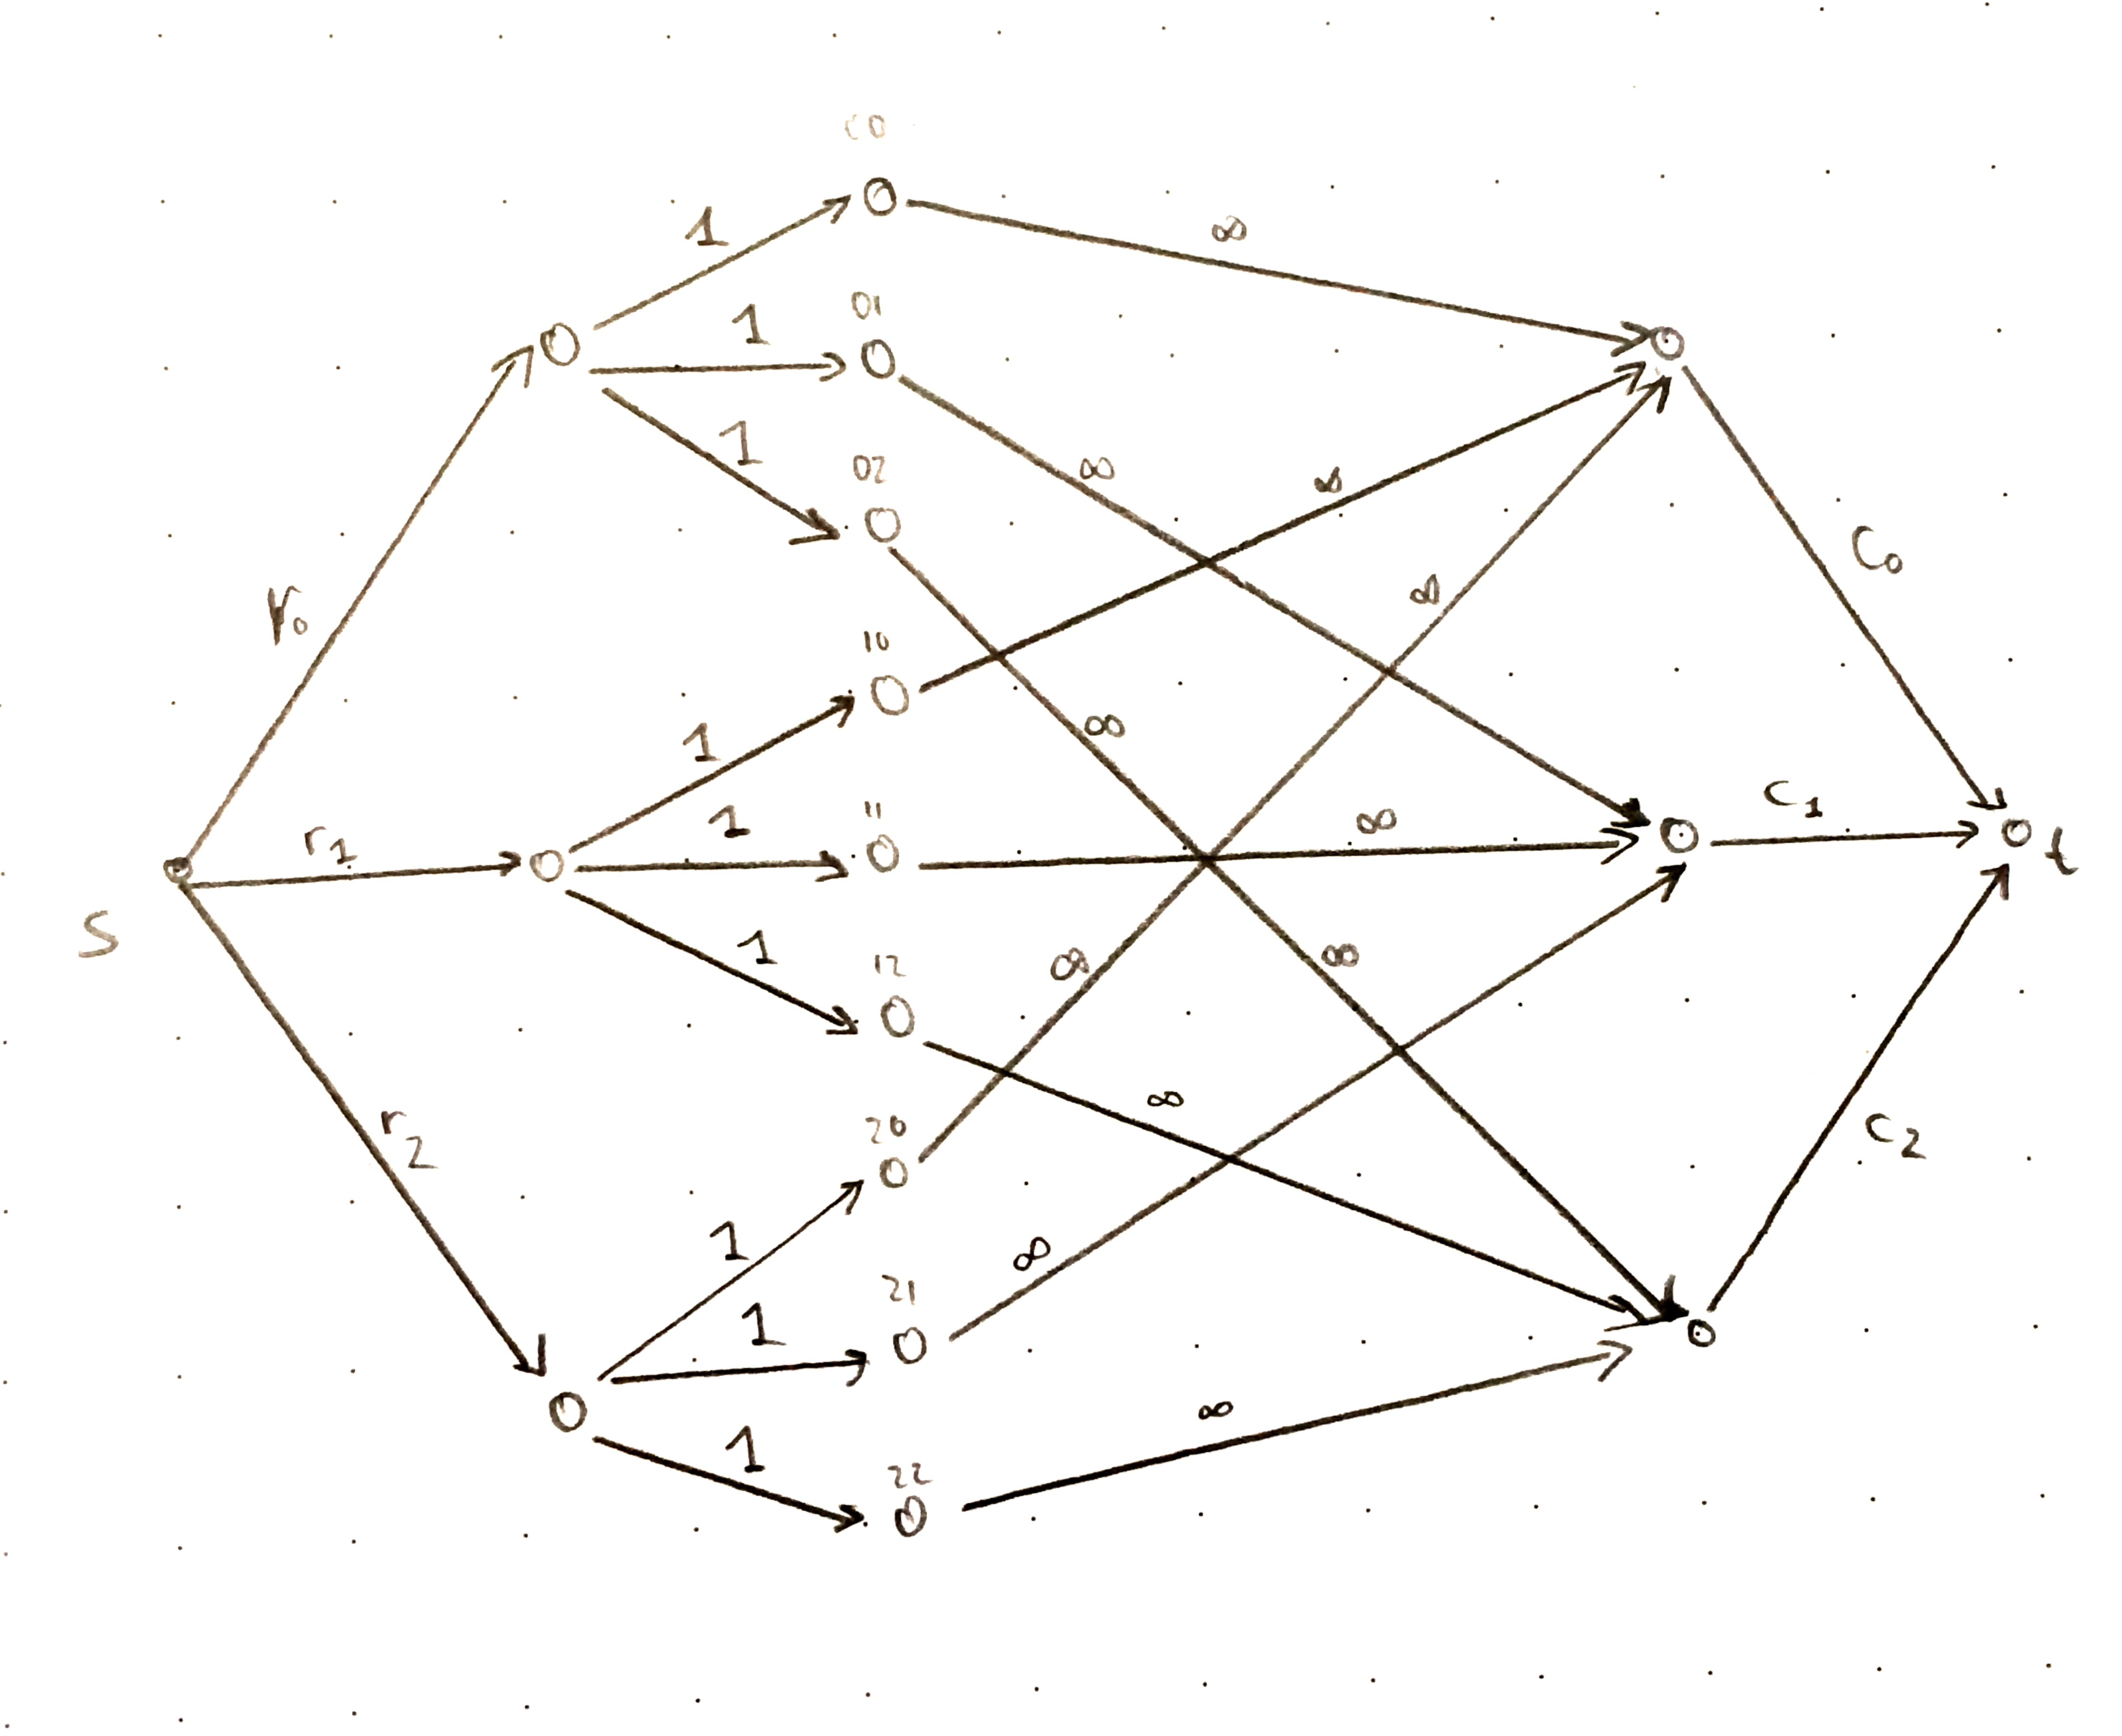
\includegraphics[width=\textwidth]{3_a.pdf}
\begin{itemize}
	\item We create a flow network for the table. The table entries can be rounded to integers by satisfying all column and row constraints iff the max flow of the graph is the sum of all column/row sums.
	\item We can reconstruct the rounding by evaluating the flow values.
	\item For every cell entry, the value can either be 0 or 1 (edges with capacity 1). A flow value of 1 means that the cell entry is 1.
	\item Edges with flow $r_i$ and $c_i$ ensure that the column/row sums are not exceeded. If the max flow value is smaller than the sum of all column/row sums, then at least one row/column sum is too small.
\end{itemize}

\subsubsection*{Graph Construction}
\begin{itemize}
	\item Create a source $s$ and a sink $t$.
	\item Create a vertex $v_{r_i}$ for every row $i$ and a vertex $v_{c_i}$ for every column $i$.
	\item Create edges $(s, v_{r_i})$ with capacities $r_i$ where $r_i$ is the row sum of row $i$.
	\item Create edges $(v_{c_i}, t)$ with capacities $c_i$ where $c_i$ is the column sum of column $i$.
	\item Create a vertex $c_{a,b}$ for every cell where $a$ is the cell's row and $b$ is the cell's column.
	\item Create edges $(v_{r_i}, c_{i,b})$ for every $b$ and every row $i$ with capacity $1$.
	\item Create edges $(c_{a,i}, v_{c_i})$ for every $a$ and every column $i$ with capacity $\infty$.
\end{itemize}

\subsubsection*{Algorithm}
\begin{itemize}
	\item Build the flow graph $G$ for the input table.
	\item Run Ford-Fulkerson on $G$ to determine the max flow.
	\item Extract the solution from the max flow\footnote{$f(e)$ is the flow value for $e$ in the maximum flow.}.
	\begin{itemize}
		\item Round $c_{a,b}$ up (use 1) if $f((v_{r_a}, c_{a,b})) = 1$.
		\item Round $c_{a,b}$ down (use 0) if $f((v_{r_a}, c_{a,b})) = 0$.
	\end{itemize}
	\item Output the rounded values $c_{a,b}$.
\end{itemize}

\subsubsection*{Proof}
\begin{itemize}
	\item \textbf{Integrality constraints:} since all capacity values are integers, Ford-Fulkerson assigns only integer flow values. Therefore, for every combination of $a$ and $b$, $c_{a,b}$ is always an integer. Having calculated the max flow, we can always extract the information whether to round a number up or down.
	\item \textbf{Rounding constraints:} since all edges $(v_{r_i}, c_{i,b})$ have a capacity of 1 and integrality is ensured, we can conclude that the max flow assigns only values 0 or 1 to each cell. Therefore, we can be sure that this algorithm does only round numbers up or down but not assign other numbers to cells\footnote{Assumption: the problem description says that all cell values are between 0 and 1. We assume, that the bounds are excluding, i.e. there is no cell with a value of 0 or 1. If this is allowed, we can adapt the algorithm to cope with this situation (see later subsection).}.
	\item \textbf{Row constraints:} for every row $i$, all $c_{i, b}$ (for all $b$) are connected to the source via edges $(s, v_{r_i})$, with a capacity of the respective row sum. Therefore, we can be sure that the sum of all rounded cells in row $i$ cannot exceed $r_i$. We also know that there is no possible rounding, if the max flow is smaller than $\sum_{i} r_i$. In that case, at least one of the edges $(s, v_{r_i})$ has a remaining capacity that was not used by the max flow. Therefore, the row sum is too small.
	\item \textbf{Column constraints:} we can make the same argument for column sums, by examining the edges $(v_{c_i}, t)$.
	\item \textbf{Summary:} the algorithm finds a valid rounding if there exists one, because all cell numbers are either rounded to 0 or 1, row and column constraints are ensured and we can extract the rounding from the max flow/residual graph after running the Ford-Fulkerson algorithm.
\end{itemize}

\subsubsection*{Runtime}
\begin{itemize}
	\item Building the graph can be done in $\mathcal{O}(n)$, where $n$ is the number of cells in the table, because we have to add $n$ vertices in the middle, $2n$ edges connecting there vertices, and $2 \sqrt{n}$ vertices for row/column sums\footnote{We assume that the number of rows and columns is equal. Even if this is not the case, this number can never exceed $n$.} together with the same number of edges connecting these vertices with the source and the sink.
	\item The Edmont-Karp algorithm, a variation of the ford fulkerson algorithm, can find the max flow in $\mathcal{O}(V E^2)$, where $V$ is the number of vertices and $E$ is the number of edges in the graph. In our case, $V = \mathcal{O}(n)$ and $E = \mathcal{O}(n)$ (see previous argument), therefore the runtime is $\mathcal{O}(n^3)$.
	\item For extracting the solution, we need to examine $n$ edges.
	\item The overall runtime of the algorithm is $\mathcal{O}(n^3)$.
\end{itemize}

\subsubsection*{Variation: Inclusive lower/upper bound}
The algorithm can be modified to support values of $0$ and $1$ inside the table. Instead of showing the exact changes necessary here, take a look at subproblem b, which is a more general problem and supports inclusive lower/upper bounds, i.e. integers as cell values.

\subsection*{Subproblem b}
\subsubsection*{Basic Idea}
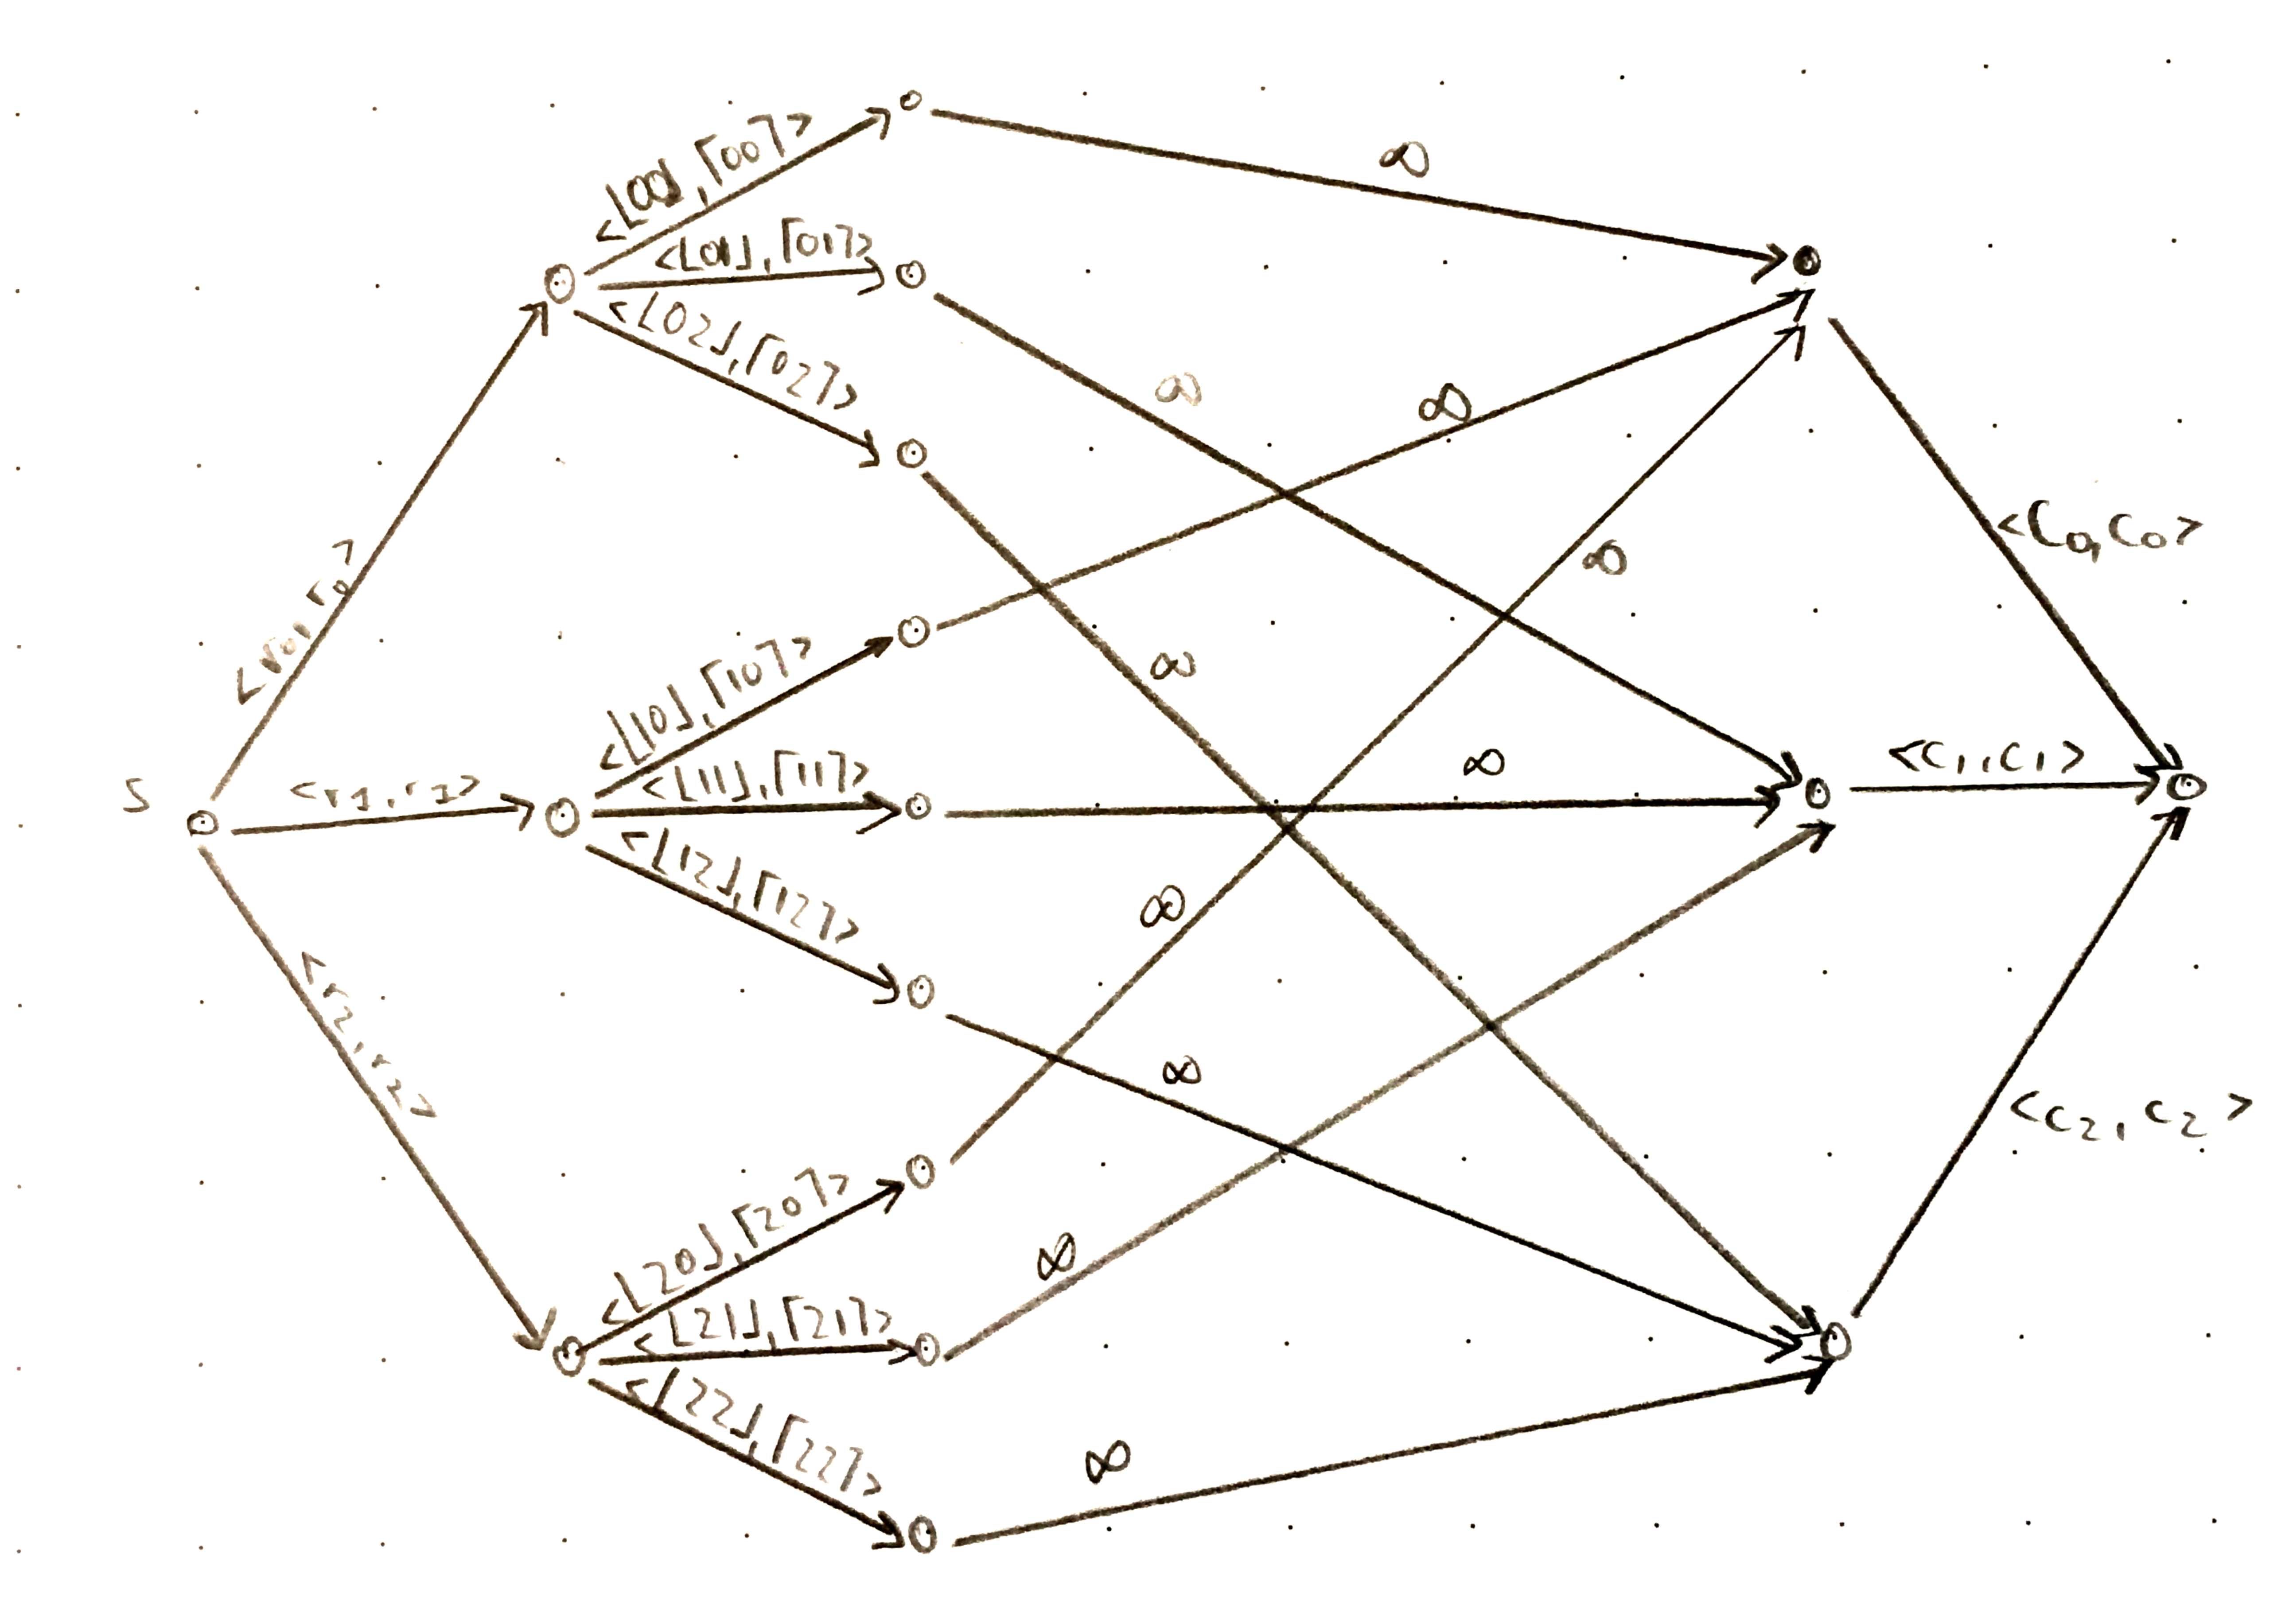
\includegraphics[width=\textwidth]{3_b.pdf}

\begin{itemize}
	\item We use a modified version of max flow that supports lower bounds on the flow values, in addition to capacity constraints. We will show how this can be reduced to the original max flow problem.
	\item The graph is similar to subproblem a, but instead of putting a capacity constraint of 1 on all edges $(v_{r_i}, c_{i, b})$, we use a lower bound of $\lfloor o_{i,b} \rfloor$ and an upper bound (capacity constraint) of $\lceil o_{i,b} \rceil$, where $o_{i,b}$ is the original value of the cell $(i, b)$ in the table.
	\item We force the connecting edges of the source and the sink to be the row/column sums by putting the same lower and upper bound of $r_i$ or $c_i$ respectively on the edge flow.
	\item The problem is solvable, if there is a flow that satisfies all constraints. Note, that the notion of a max flow does not make sense here, because all of $s$'s outgoing edges are forced to be a specific value.
\end{itemize}

\subsubsection*{Graph Construction}
\begin{itemize}
	\item Build the graph exactly as in subproblem a but with the following modifications.
	\item For every edge $(v_{r_i}, c_{i,b})$, use $\lfloor o_{i,b} \rfloor$\footnote{In the graph illustration, we just wrote $00$ instead if $o_{0,0}$.} as a lower bound and $\lceil o_{i,b} \rceil$ as an upper bound.
	\item For every edge $(s, v_{r_i})$, use $r_i$ as a lower and as an upper bound.
	\item For every edge $(v_{c_i}, t)$, use $c_i$ as a lower and as an upper bound.
\end{itemize}

\subsubsection*{Algorithm}
We assume at this point that we have an algorithm that can solve the flow problem\footnote{How this actually works is shown in one of the next subsections.}, i.e. assign flow values to all edges, such that all constraints are satisfied. We are not looking for a max flow here, but only some assignment, that satisfies flow conservation, capacity constraints and minimum flow constraints.

\begin{itemize}
	\item Build the flow graph $G$ for the input table.
	\item Assign flow values to the graph, such that all constraints are satisfied, using the algorithm described in the next subsections.
	\item Extract the solution from the flow values.
	\begin{itemize}
		\item Round $c_{a,b}$ up if $f((v_{r_a}, c_{a,b})) = \lceil o_{a,b} \rceil$.
		\item Round $c_{a,b}$ down if $f((v_{r_a}, c_{a,b})) = \lfloor o_{a,b} \rfloor$. 
	\end{itemize}
	\item Output the rounded values $c_{a,b}$.
\end{itemize}

\subsubsection*{Proof}
\begin{itemize}
	\item The proof is similar to subproblem a's proof.
	\item \textbf{Integrality constraints:} see subproblem a.
	\item \textbf{Rounding constraints:} similarly to subproblem a, we assign only the values $\lfloor o_{a,b} \rfloor$ or $\lceil o_{a,b} \rceil$, because these are the lower/upper bounds, their difference is at most 1 and  we already showed integrality. Note, that this version of the algorithm allows values in the table to be integers (in contrast to the algorithm shown in subproblem a). Therefore, we can use this algorithm to solve subproblem a where the lower/upper bounds are inclusive, i.e. 0 and 1  are allowed as table cell values.
	\item \textbf{Row constraints:} we enforce that the sum of the cells per row is the row sum for that row. Therefore, we do not have to calculate the flow value of the graph. For a single row it is sufficient to check, whether the upper/lower bounds are satisfied. These constraints must be satisfied, because this is ensured by the algorithm that we ran in the second step.
	\item \textbf{Column constraints:} the same argument can be made for column constraints.
\end{itemize}

\subsection*{Reduction to Max-Flow}
The following graph shows how to reduce the previous graph with lower bounds to the classical max flow problem (for a smaller example).

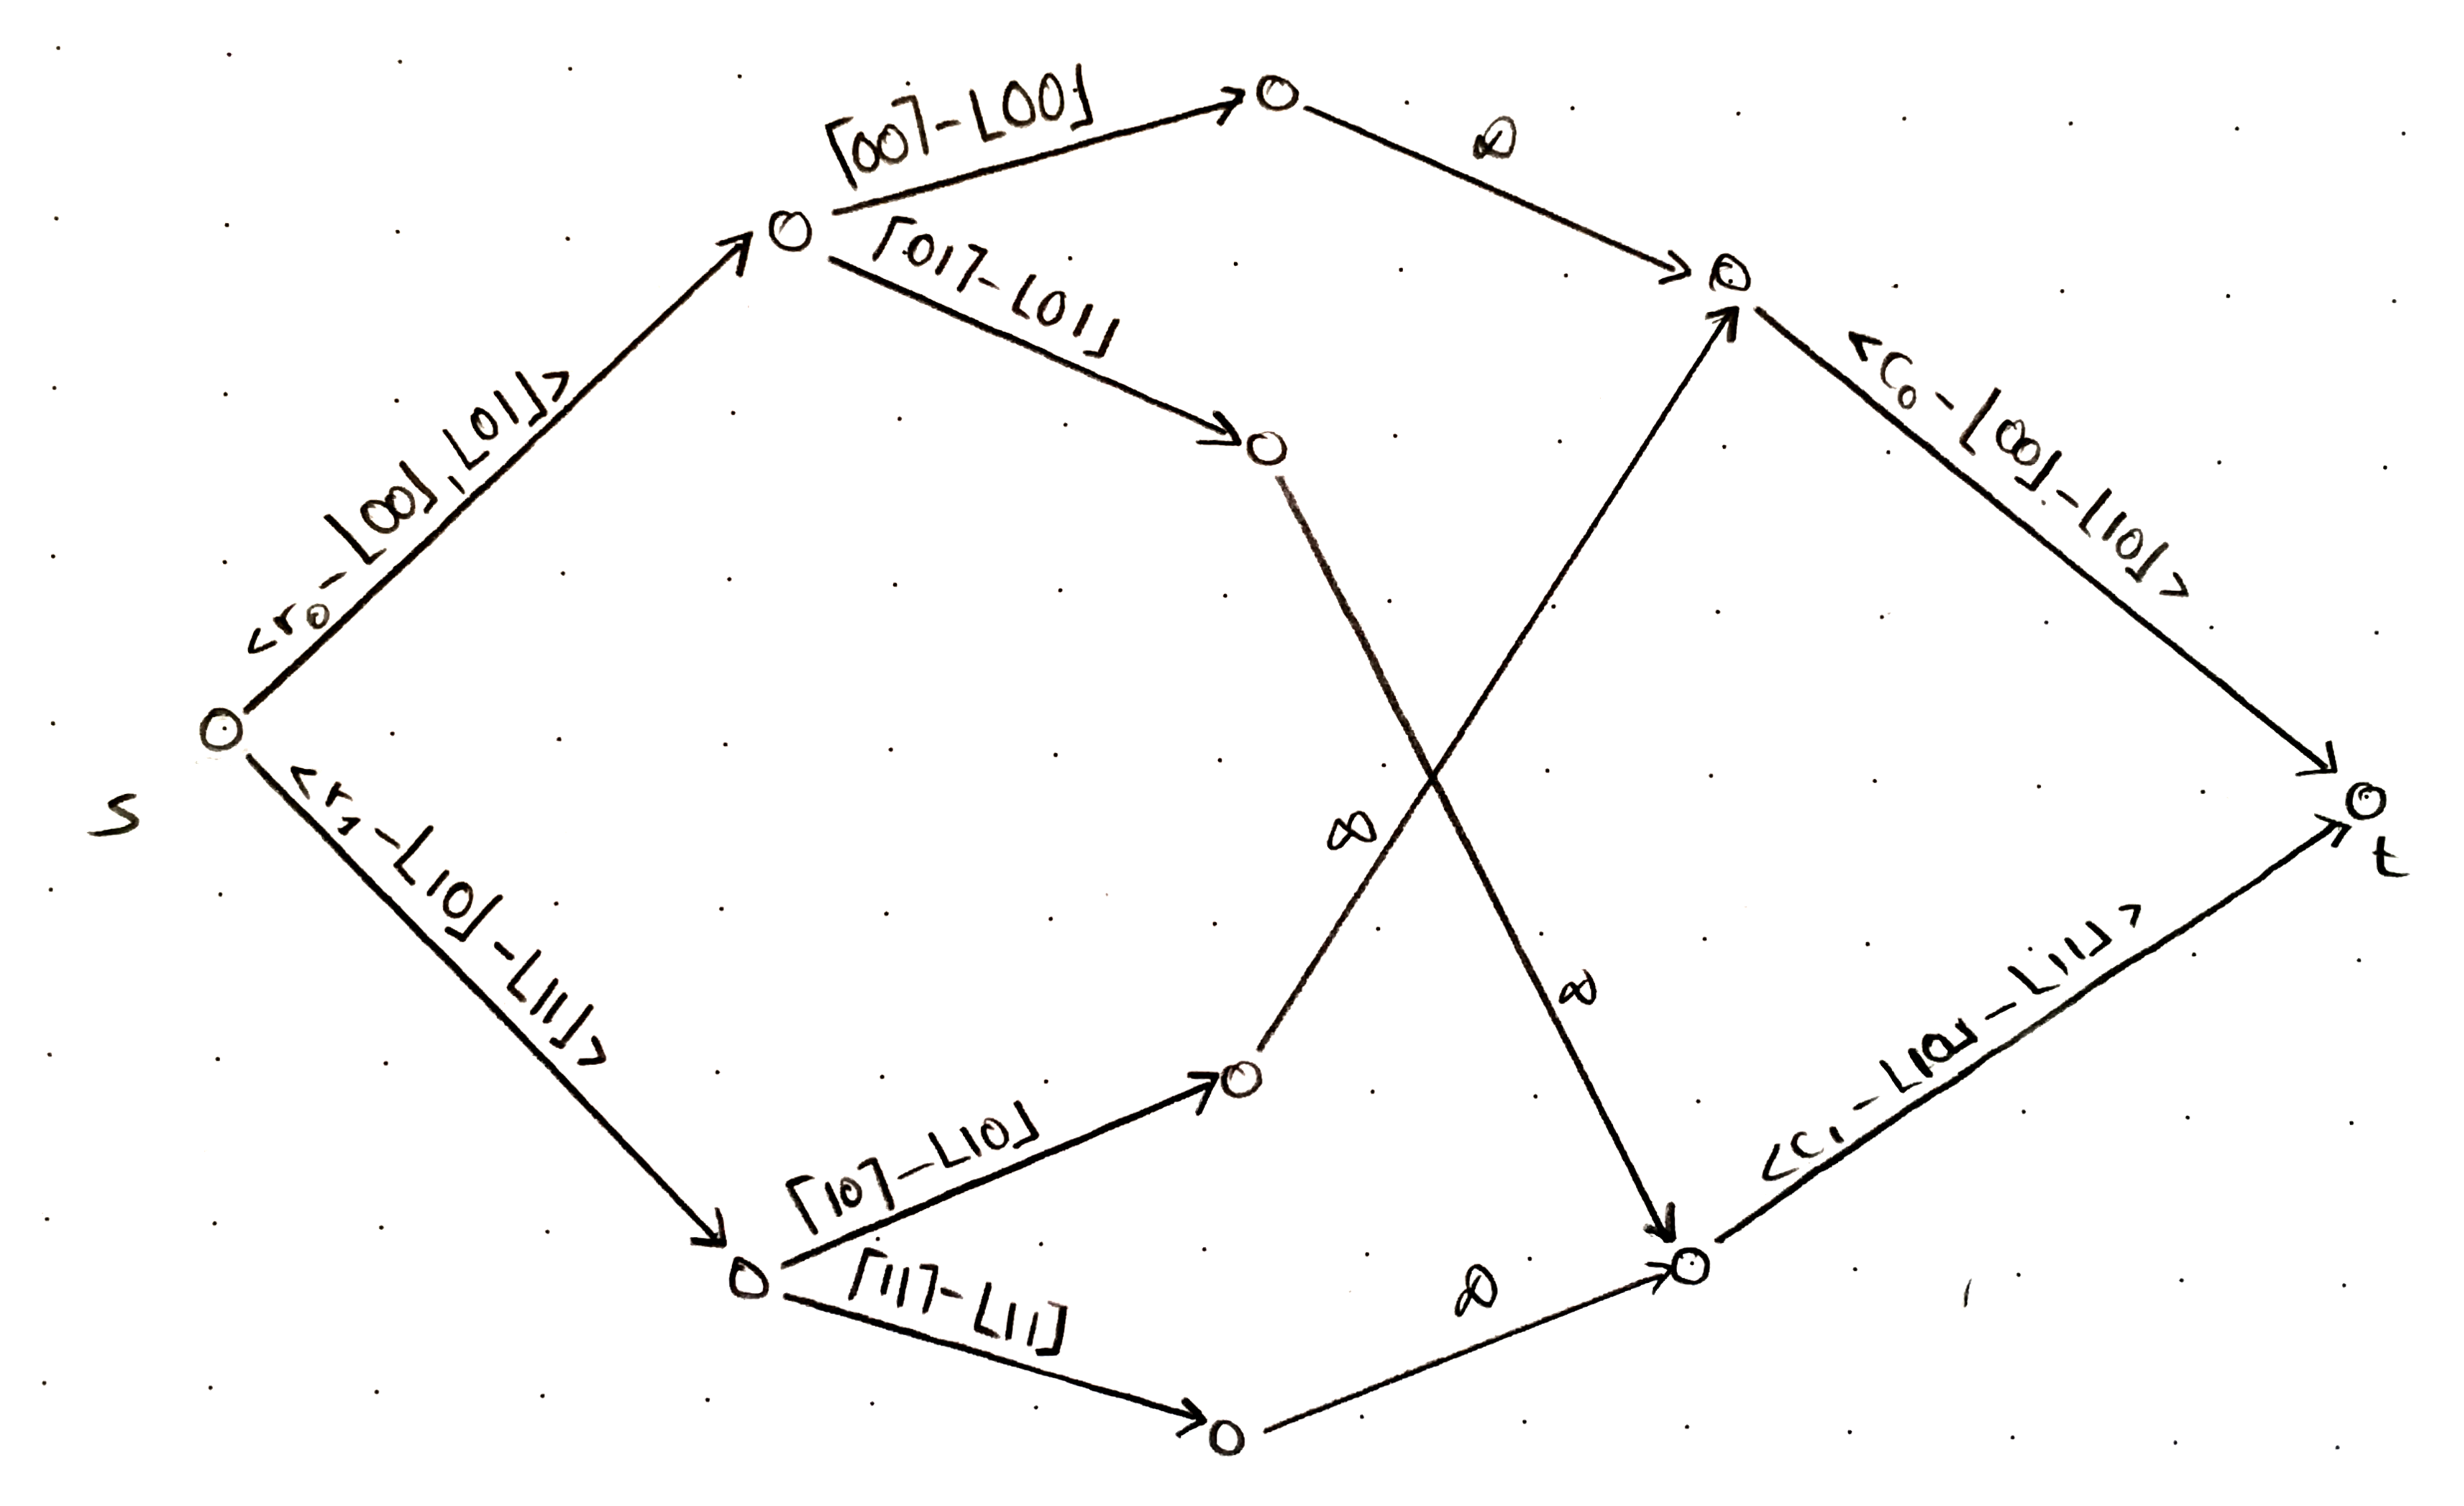
\includegraphics[width=\textwidth]{3_b_2.pdf}

\begin{itemize}
	\item For every edge $(v_{r_a}, c_{a,b})$ with a lower bound of $l$ and an upper bound of $r$, remove $l$ from every edge on every s-t path that uses this edge. Note, that there is only one that path. The lower bound is now 0, thus we removed a lower bound.
	\item The resulting graph still has edges $(s, v_{r_a})$ and $(v_{c_b}, t)$ that enforce a specific value (by using the same upper and lower bound). We remove the lower bound.
	\item If and only if the resulting graph has a max flow of $\sum_{i} r_i - \sum_{a,b} \lfloor o_{a,b}\rfloor$, then the problem is solvable. By subtracting the lower bound from every path, we could still satisfy the constraints in the original graph by just adding the lower bound to every edge on this path. When we achieve the stated max flow value, then all of $s$'s outgoing edges and all of $t$'s incoming edges have a residual (forward) capacity of 0, i.e. there is no capacity left. Therefore, after adding the subtracted values again, we would flow the row/column sums using these edges. This is necessary for a valid solution.
	\item This is how we construct the original flow values for edges $(v_{r_a}, c_{a,b})$: if flow in the new graph is 0, then we flow the lower bound. If the flow is 1, then we flow the upper bound. Note, that the difference between upper and lower bound is at most 1.
\end{itemize}

\subsubsection*{Runtime}
The runtime of this problem is the runtime of problem a plus the runtime required for transforming the graph. Changing the edge capacities/lower bounds can be done in $\mathcal{O}(E)$, where $E$ is the number of edges. From the argument in subproblem a we know that there are $\mathcal{O}(n)$ edges. Therefore, the overall runtime is still $\mathcal{O}(n^3)$.

\subsection*{Subproblem c}
Note, that subproblem a is just a special case of subproblem b. Therefore, if we prove the assumption for subproblem b, we have automatically proven it for subproblem a.

We prove that the max flow/min cut in the modified graph without lower bounds is always $\sum_i r_i - \sum_{a,b} \lfloor o_{a,b} \rfloor$. In that case, there is always a valid solution for the graphs with lower bounds (see argumentation in subproblem b). Therefore, we can always round the numbers, such that the constraints are satisfied.

\begin{itemize}
	\item We claim that $C=(A,B)$, $A=\{s\}$, $B=V-A$ is a min cut.
	\item If we add one of the vertices $v_{r_a}$, then the cut capacity can only become bigger (or stay the same). We can prove this by examining the change of the cut capacity: $(\sum_i \lceil o_{a,i} \rceil - \lfloor o_{a,i} \rfloor) - (r_a - \sum_i \lfloor o_{a,i} \rfloor) = \sum_i (\lceil o_{a,i} \rceil) - r_a$. We know that this term must be positive, because by definition $r_a = \sum_i o_{a,i}$ and the ceiled value is always bigger than or equal to the value.
	\item If we add another vertex $c_{a,b}$ in addition, we also have to add the vertex $v_{c_b}$, because the connecting edge has infinite capacity.
	\item If we additionally add another vertex $v_{c_b}$, we can not compensate this. We can prove this by examining the total change of adding both vertices: $c_b - \sum_i \lfloor o_{i, b} \rfloor + \sum_{i \not= b} (\lceil o_{a,i} \rceil - \lfloor o_{a,i} \rfloor) - (r_a + \sum_i \lfloor o_{a,i} \rfloor) \geq 0$ (expand $r_a$ and $c_b$ similarly to previous part).
	\item Therefore, we have no way of achieving a smaller minimum cut. Note, that the cut $C=(A,B)$ with $B=\{t\}$, $A=V-B$ has the same minimum cut value. 
\end{itemize}

\section*{Problem 5}
\subsection*{Basic Idea}
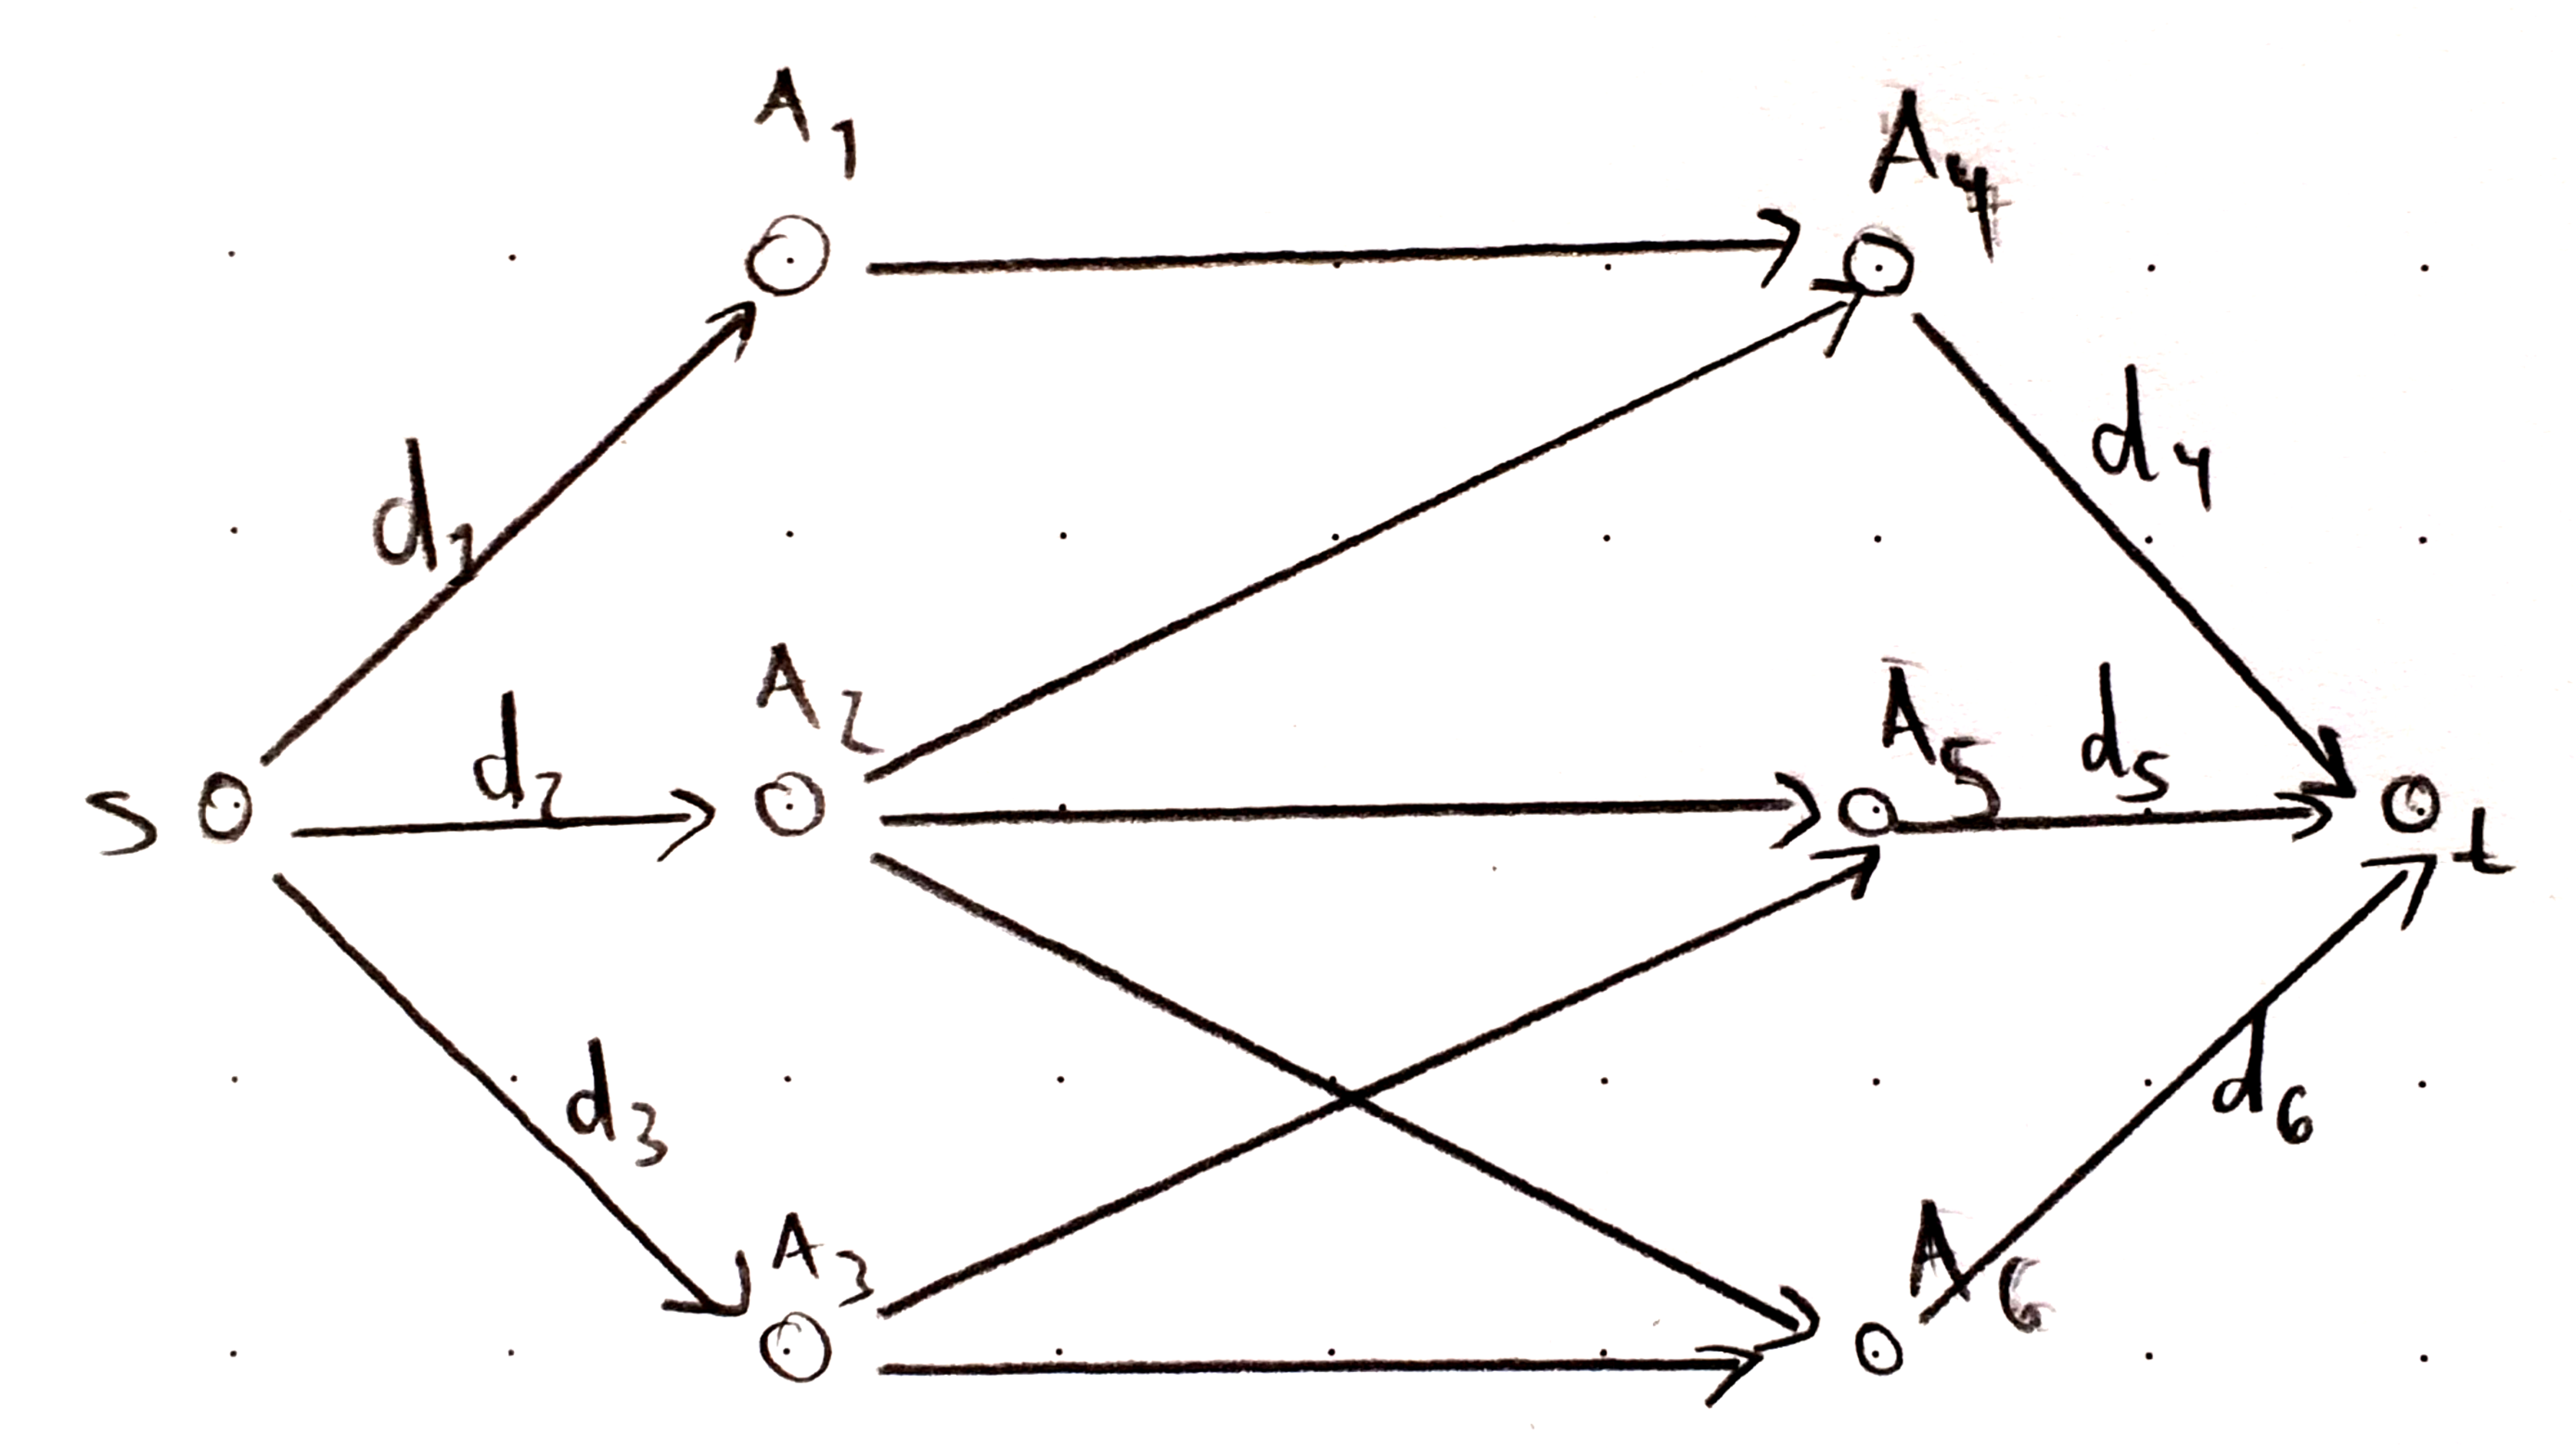
\includegraphics[width=\textwidth]{5.pdf}

\begin{itemize}
	\item We generate a flow graph as illustrated in the example above.
	\item The middle part of the graph (everything without $s$ and $t$) is the original graph, but with directed edges. The capacities for these edges are 1\footnote{note, that we can arrange the vertices in such a way because the graph is bipartite.}.
	\item We connect the left vertex set with the source and give each each edge $(s, A_i)$ a capacity of $d_i$, where $d_i$ is the degree of $A_i$ in the spanning subgraph. We do the same for the right vertex set and the sink.
	\item There exists such a spanning subgraph, if and only if the max flow of this graph is the sum of all $d_j$, where $j$ is the set of vertices on the left side.
	\item We can extract the spanning subgraph by taking only the edges with a flow of 1.
	\item We can partition the bipartite graph into two vertex sets with DFS. Note, that a graph is bipartite if and only if its chromatic number is 2. Therefore, the DFS can just assign the opposite color when exploring a new vertex.
\end{itemize}

\subsubsection*{Graph Construction}
\begin{itemize}
	\item Add a source $s$ and a sink $t$.
	\item Let $V=(V_1, V_2)$ be the original vertex set.
	\item Add all vertices $V$.
	\item Add an edge $(a, b)$ for all $a \in V_1$, $b \in V_2$, $\{a,b\} \in E$ with capacity 1.
	\item For all $a \in V_1$, add an edge $(s, a)$ with capacity $d_a$. For all $b \in V_2$, add an edge $(b, t)$ with capacity $d_b$.
\end{itemize}

\subsubsection*{Necessary Conditions}
\begin{itemize}
	\item $G=(V,E)$ is bipartite, therefore we can write $V=(V_1, V_2)$. $|V_1| = |V_2|$ is a necessary condition. Otherwise, we would require $V_1$ to have more outgoing edges than $V_2$ has incoming edges or $V_2$ to have more incoming edges than $V_1$ has outgoing edges.
\end{itemize}

\subsubsection*{Algorithm}
\begin{itemize}
	\item Split $V$ in sets $V_1$ and $V_2$ with $V_1 \cap V_2 = \emptyset$ and $\forall a \in V_1, b \in V_2: \{a, b\} \not\in E$ using DFS: when exploring a new node, assign the node the opposite color of the current node (there are only two colors). The initial node can be an arbitrary color. Split $V$ into $V_1$ and $V_2$ according to their colors.
	\item Build the flow network.
	\item Calculate the max flow with Ford-Fulkerson algorithm.
	\item If the max flow is smaller than $\sum_{i \in V_1} d_i$, then output \emph{no solution}.
	\item Else, output all edges $(a,b)$ with $a \not= s$ and $b \not= t$ and $f((a,b)) = 1$.
\end{itemize}

\subsubsection*{Proof}
\begin{itemize}
	\item \textbf{Integrality constraints:} Ford-Fulkerson generates a max flow with integer flow values, because all capacity values are integers. Therefore, the flow values for edges $(a,b)$ with $a \in V_1$ and $b \in V_2$ are 0 or 1 and we can extract the solution from that.
	\item \textbf{Degree constraints:} For every vertex $a \in V_1$ in the left vertex set, we cannot use more than $d_a$ outgoing edges, because the capacity of the connecting edge $(s, a)$ is $d_a$. Similarly, for every vertex $b \in V_2$, we cannot use more than $d_b$ incoming edges. When the max flow is $\sum_{a \in V_1} d_a = \sum_{b \in V_2} d_b$, we can be sure that we used $d_i$ edges for every vertex $V_i$ (because of flow conversation).
	\item We can always partition $V$ into $V_1$ and $V_2$, because a graph is bipartite if and only if it is two-colorable.
\end{itemize}

\subsubsection*{Runtime}
\begin{itemize}
	\item Generating sets $V_1$ and $V_2$ with DFS: $\mathcal{O}(|V| + |E|)$.
	\item Build the flow network. This involves adding $|V|$ connecting edges and setting capacity constraints for $|E|$ edges. Therefore, the runtime is bounded by $\mathcal{O}(|V| + |E|)$
	\item Generating the max flow with the Edmonds-Karp algorithm in $\mathcal{O}(|V||E|^2)$
	\item Extracting the solution by examining $\mathcal{O}(|E|)$ edges.
	\item The overall runtime is $\mathcal{O}(\max \{ |V| + |E|, |V||E|^2 \})$.
\end{itemize}

\section*{Problem 1}
\subsection*{Basic Idea}
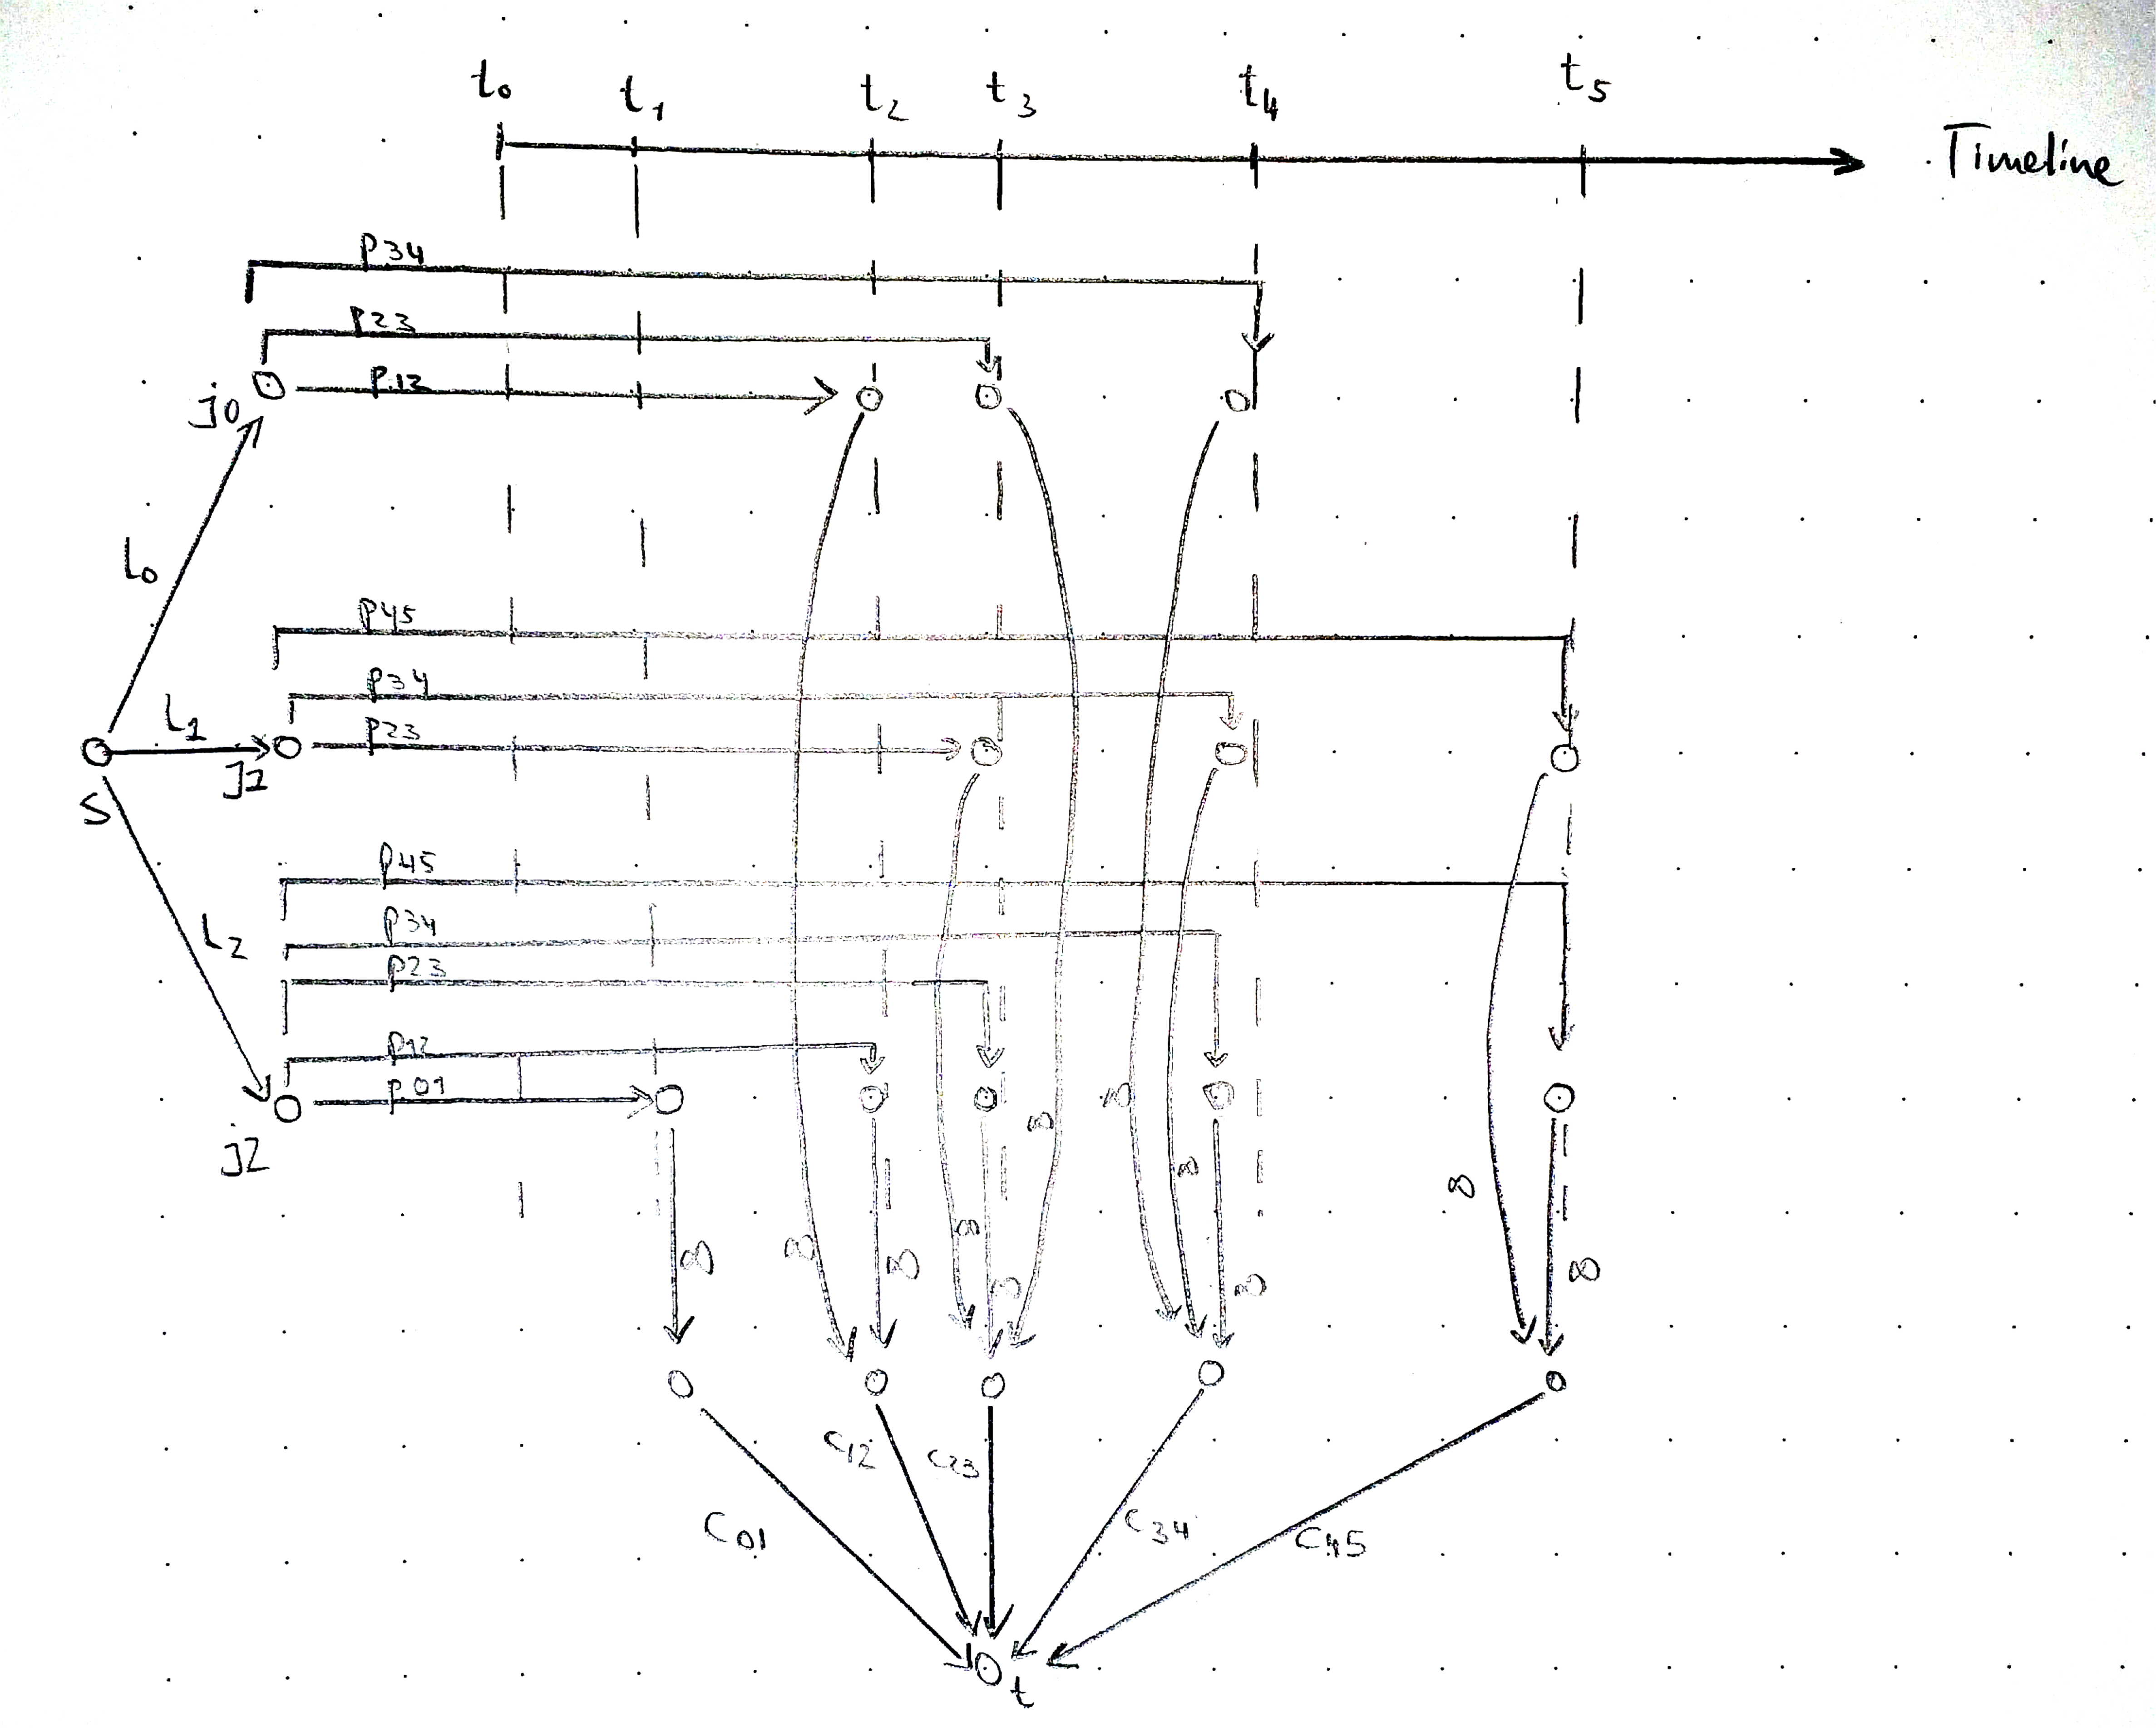
\includegraphics[width=\textwidth]{1.pdf}

\begin{itemize}
	\item We precalucate a set of time points $t_i$ where \emph{something} changes, i.e. where a processor becomes available, a processor vanishes or a job becomes available.
	\item At every $t_i$, we redistribute a subset of all available jobs onto the available processors.
	\item For every time interval $t_{i-1}$ to $t_i$, we precalculate the processor capacity $c_{i-1, i}$, i.e. the processing power of all available processors. For instance, if two processors are available in the interval $t_{i-1}$ to $t_i$ with length $[4.5; 6)$, then the processor capacity for this interval is $c_{i-1, i} = 3$.
	\item We connect every job with the source. The capacity of the edge is the duration of the job.
	\item We connect every job with every possible end point of a time interval (by creating new vertices $k$ for every job). For instance, if job 1 is available from $t_2$ to $t_5$, we connect it with $t_3$, $t_4$ and $t_5$, because it could run in any one of the intervals 2-3, 3-4, 4-5. Each edge's capacity is the length of the interval ($p_{i-1,i}$). This ensures that we do no use more processing power than one processor can provide in this interval.
	\item For every time point $t_i$, we connect the vertices of all jobs at this time point with an intermediate vertex. This vertex is connected to the sink with a capacity value of $c_{i-1, i}$. This ensures that we do not schedule too many processes.
	\item The problem has a solution if and only if the max flow is $\sum_i l_i$, where $l_i$ is the length of job $i$. By examining the flow values of the edges with capacities of $p_{a,b}$ we can determine in which intervals a job is supposed to run. To generate a concrete schedule, we have to do a post-processing step.
\end{itemize}

\subsection*{Graph Construction}
\begin{itemize}
	\item Create a source $s$ and a sink $t$.
	\item Create a vertex $j_i$ for every job $i$ and connect it to the source with a capacity of $l_i$ (direction: towards $j_i$).
	\item For every job $i$, create a set of vertices $k_{i, j}$, where $i$ is available in an interval $t_{j-1}$ to $t_j$. I.e. the smallest $t_{j-1}$ represents the time point where $i$ becomes available and the largest $t_j$ represents the deadline for the job.
	\item Connect every $j_i$ with all $k_{i, m}$ with a capacity that is the duration of the interval $m-1$ to $m$ (in other words: the processing power of one processor in that time interval).
	\item Create vertices $w_i$ for every time point i. These vertices sum up all the work that is done in one interval.
	\item Create edges $(k_{i, j}, w_j)$ for all jobs $i$, with  capacity of $\infty$.
	\item Create edges $(w_i, t)$ with a capacity of $c_{i-1, i}$.
\end{itemize}

\subsubsection*{Algorithm}
\begin{itemize}
	\item Calculate all time points $t_i$ by creating list of all times when a processor becomes available or vanishes and when a job becomes available. Sort that list.
	\item For every time interval $t_{i-1}$ to $t_i$ calculate the processor capacity by checking which processors are available in every interval and multiplying this number with the length of the interval.
	\item Generate the flow graph $G$. If the max flow is smaller than $\sum_i l_i$, return \emph{no solution}.
	\item Calculate the max flow of $G$ with the Ford-Fulkerson algorithm.
	\item For every interval $t_{i-1}$ to $t_i$ and every job $m$, generate a mapping of running times. The runtime of job $m$ in that interval is the flow value of the edge between the vertices $j_m$ and $k_{m,i}$.
	\item For every interval, generate a concrete schedule: use the algorithm described below.
\end{itemize}

\begin{algorithmic}
	\State $\mathit{cpu} \gets 1$
	\State $\mathit{time} \gets 0$
	\ForAll{$(\mathit{job}, \mathit{runtime}) \in \mathit{mapping}$}
		\If{$\mathit{time} + \mathit{runtime} \leq \mathit{intervalLength}$}
			\State $\mathit{schedule}(\mathit{job}, \mathit{cpu}, \mathit{time}, \mathit{time} + \mathit{runtime})$
			\State $\mathit{time} \gets \mathit{time} + \mathit{runtime}$
		\Else
			\State $\mathit{schedule}(\mathit{job}, \mathit{cpu}, \mathit{cpu}, \mathit{intervalLength})$
			\State $\mathit{time} \gets \mathit{runtime} - (\mathit{intervalLength} - \mathit{time})$
			\State $\mathit{cpu} \gets \mathit{cpu} + 1$
			\State $\mathit{schedule}(\mathit{job}, \mathit{cpu}, 0, \mathit{time})$
		\EndIf
	\EndFor
\end{algorithmic}

The function $\mathit{schedule}$ schedules a job on a specific processor for a given time span (start time and end time). Note, that the algorithm might schedule a job on two different processors, but a single job is never run in parallel on multiple processors, because the length of a job run ($\mathit{runtime}$) is never bigger than the length of the interval\footnote{See proof for more details.}.

\subsection*{Proof}
\begin{itemize}
	\item The number of processors stays constant in every interval and no new jobs are added. Therefore, we can assume that we have a single processor with a bigger amount of computing power, as long as no job gets scheduled for more than the interval length (parallel computation is not allowed). We show later, that we can then always generate a concrete valid scheduling.
	\item Every job is scheduled: if the max flow is $\sum_i l_i$, then every job $i$ runs exactly for a time of $l_i$ during a number of intervals, because due to flow conservation the computing time must be delegated to these intervals.
	\item Every interval $t_{i-1}$ to $t_{i}$ cannot get more than $c_{i-1, i}$ computing load (capacity constraints on edges that lead to $t$). In addition, no job in that interval is scheduled longer than the interval length. Therefore, we can always generate a concrete schedule for every interval by scheduling the jobs after each other and choosing a new processor once the current processor has no computing time left in the current interval. The rest of the current job might be scheduled on the new processor, resulting in two different run time spans for a single job. However, these two spans can never overlap, because the total computing time for a single job does not exceed the interval length because of the capacity constraints $p_{i-1, i}$.
\end{itemize}

\subsection*{Runtime}
Let $r$ be the number of processors and $e$ be the number of jobs.

\begin{itemize}
	\item Calculating points $t_i$: the list contains $2r + e$ time points. Therefore, sorting takes $\mathcal{O}((2r+e) \log (2r + e))$ time.
	\item Calculating the processor capacity for every time interval: there are $2r+e-1$ time intervals and for every interval, we need to check $r$ processors. Therefore, this takes $\mathcal{O}(r^2 + er)$ time.
	\item Generate the graph $G$: we create vertices for every job, every time interval and a vertex for some time intervals in every job. Therefore, we create $\mathcal{O}(er)$ vertices and no more than $\mathcal{O}(e^2 r^2)$ edges (assuming that we generate a node between every pair of vertices).
	\item Calculate the max flow with the Edmonds-Karp algorithm: since we have $\mathcal{O}(er)$ vertices and $\mathcal{O}(e^2 r^2)$ edges, the Edmonds-Karp algorithm runs in $\mathcal{O}(e^5 r^5)$.
	\item Generating the concrete schedule from the mapping: in the worst case, every job is scheduled very shortly in every interval, therefore we have to examine $\mathcal{O}((2r + e) \cdot e) = \mathcal{O}(re + e^2)$ job time spans.
	\item The overall runtime complexity of the algorithm is therefore $\mathcal{O}(e^5 r^5)$ ($e \geq 1$ and $r \geq 1$)\footnote{There is most likely a much better upper bound, but the problem description just asked for a polynomial algorithm.}. Therefore, the algorithm is polynomial.
\end{itemize}

\section*{Problem 2}
\subsection*{Relation to Baseball Elimination}
\begin{itemize}
	\item This problem is related to the Baseball elimination problem and we use a similar flow graph to solve it.
	\item Every vertex in the graph corresponds to a baseball team and every edge corresponds to a game to be played between two teams.
	\item No team has won a game so far and every team plays against another team only once.
	\item A subset of teams $S$ (vertices) can eliminate another team $t$, if its number of remaining games against each other divided by $|S|$ is greater than the games to be played by $t$ (we call that number $r_t$), because in that case at least one team in $S$ must have more than $r_t$ wins.
	\item Apply this idea to the graph cohesiveness problem: a set of vertices $S$ can eliminate another vertex $t$, if $\frac{e(S)}{|S|} > d_t$, where $d_t$ is the degree of vertex $t$.
\end{itemize}

\subsection*{Subproblem a}
\subsubsection*{Basic Idea}
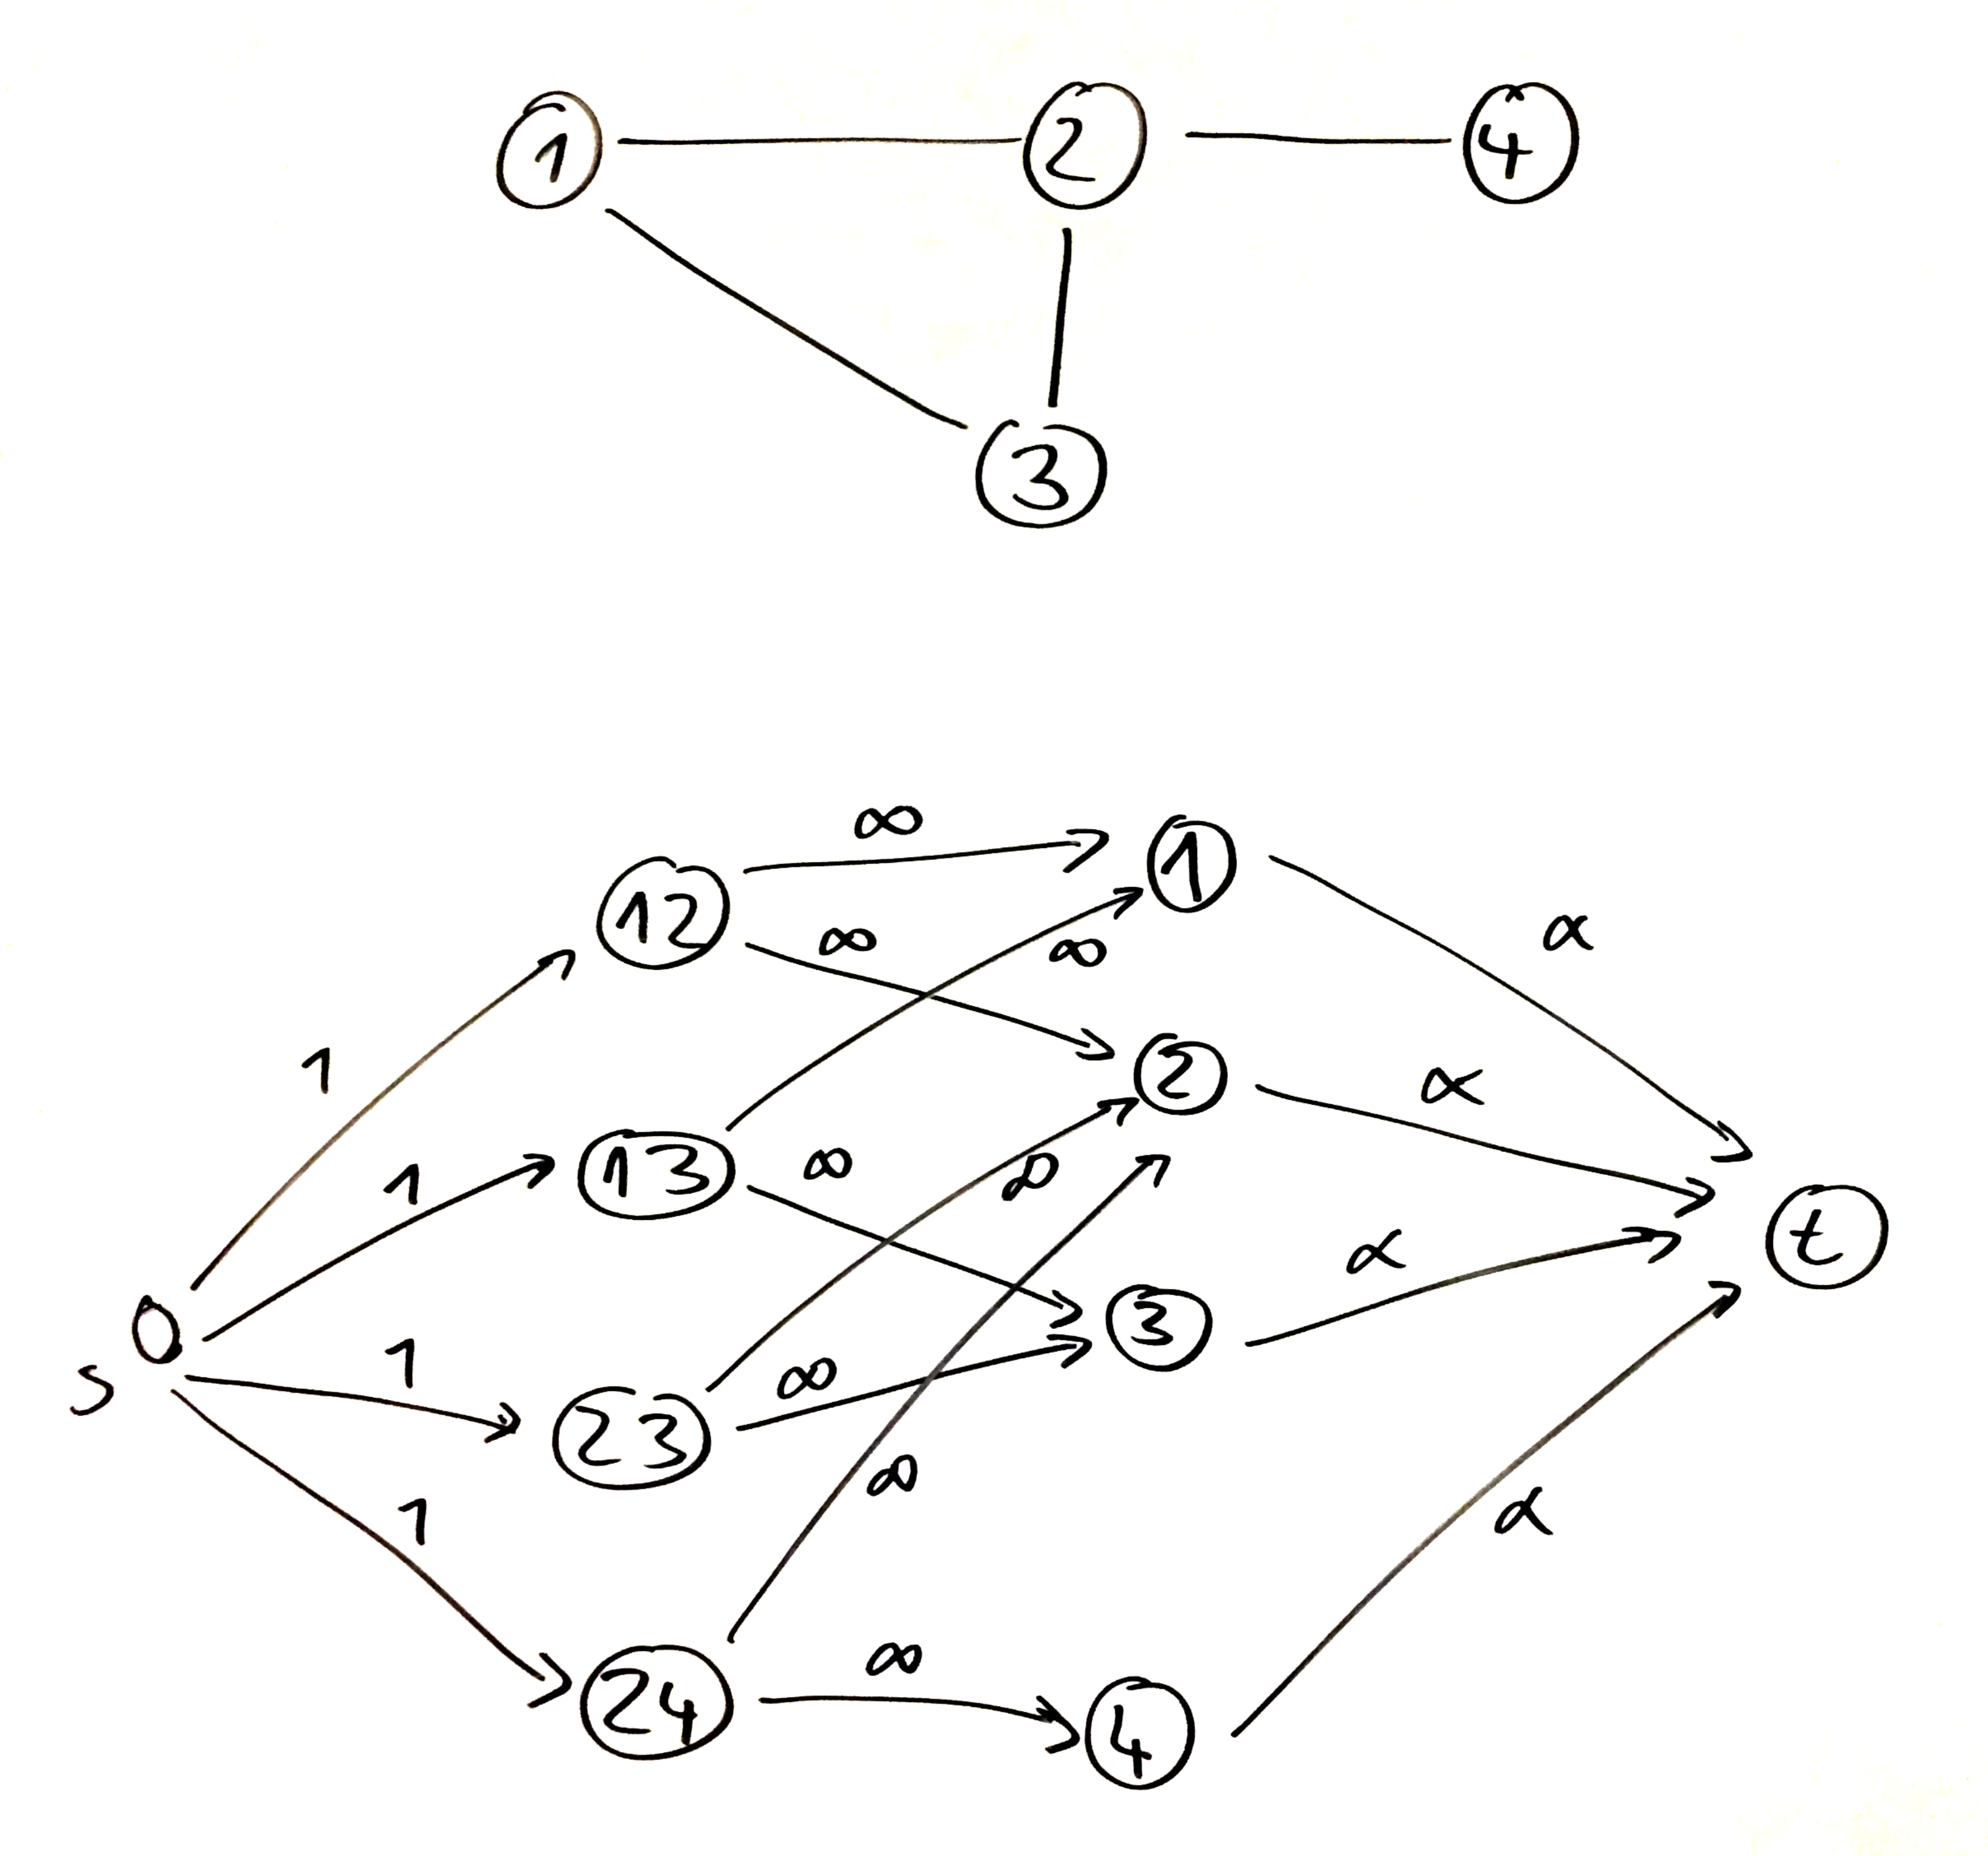
\includegraphics[width=\textwidth]{2.pdf}
\begin{itemize}
	\item We build a flow graph as shown in the figure above. There is a subset $S$ with a cohesiveness bigger than $\alpha$ iff the max flow value is smaller than $|E|$
	\item Let the vertices $ab$ on the left side represent matches and the vertices $a$ on the right side represent teams. Let every team have zero wins and every match $ab$ happen exactly once if the vertex is present. If the max flow value is smaller than $|E|$, this means that not all wins of the $|E|$ matches can be distributed in such a way that no team that has (only) $\alpha$ matches left gets eliminated.
	\item If a team with $\alpha$ matches left gets eliminated, there must be a subset $S$ with $\frac{e(S)}{|S|} > \alpha$ (same argument as lemma 7.59 in the text book). 
	\item The fact whether such a subset $S$ exists, changes only for discrete values of $\alpha$. There is a subset $S$ with $\frac{e(S)}{|S|} \geq \alpha$ iff the max flow is smaller than $|E|$ for the next smaller value of $\alpha$.
\end{itemize}

\subsubsection*{Graph Construction}
\begin{itemize}
	\item Add a source $s$ and a sink $t$.
	\item For every vertex $v_i$ in the original graph, add a vertex $v_i$.
	\item For every edge $(v_i, v_j)$ in the original graph, add a vertex $v_{ij}$.
	\item For every vertex $v_{ij}$ in the new graph, add an edge $(s, v_{ij})$ with capacity $1$.
	\item For every vertex $v_{ij}$ in the new graph, add two edges $(v_{ij}, v_i)$ and $(v_{ij}, v_j)$ with capacity $\infty$.
	\item For every vertex $v_i$ in the new graph, add an edge $(v_i, t)$ with capacity $\alpha$.
\end{itemize}

\subsubsection*{Algorithm}
Note, that the fact whether a subset $S$ with $\alpha \geq \frac{e(S)}{|S|}$ exists, changes only at discrete values of $\alpha$. The upper part of the fraction must be an integer value in $[0; |E|]$ (we cannot have more than $|E|$ edges). The lower part of the fraction must be an integer value in $[0; |V|]$ (we cannot have more than $|V|$ vertices). We can show that the difference between two different values $\alpha_1$, $\alpha_2$ must be at least $\frac{1}{n^2}$\footnote{$n = |V|$.}.

$$ \alpha_1 - \alpha_2 = \frac{a_1}{b_1} - \frac{a_2}{b_2} = \frac{a_1 b_2 - a_2 b_1}{b_1 b_2} $$

We know that the upper part of the fraction must be an integer $i$ with $|i| \geq 1$ and the lower part of the fraction can never be greater than $n^2$, because both $b_1$ and $b_2$ are bounded by $n$. Therefore, $|\alpha_1 - \alpha_2|$ must be at least $\frac{1}{n^2}$.

\begin{itemize}
	\item Calculate the next smaller value $\alpha' = \alpha - \frac{1}{n^2}$  
	\item Build the flow graph $G'$ based on the graph $G$ as described above with $\alpha'$.
	\item Calculate the maximum flow value with the Ford-Fulkerson algorithm.
	\item If the maximum flow value is smaller than $|E|$: output $\mathit{true}$, otherwise output $\mathit{false}$.
\end{itemize}

\subsubsection*{Proof}
Let us assume that the max flow value for the graph is greater or equal to $|E|$. In that case, all matches, represented by edges $(s, v_{i,j})$, can distributed to teams (represented by $v_i$) in such a way that no team has more than $\alpha$ wins. Therefore, no subset of teams can eliminate a team that has $\alpha$ games left. Therefore, no subset of teams of size $|S|$ can have more than $\alpha |S| = e(S)$ matches (represented by that number of edges) left. This means, that there cannot be a subset $S$ with $\alpha < \frac{e(S)}{|S|}$.

Let us assume that the max flow for the graph is lower than $|E|$. In that case, not all matches can be distributed to teams in such a way that no team has more than $\alpha$ wins. Therefore, at least one team must have more than $\alpha$ wins. According to lemma 7.59 (that we also proved in the lecture), we can find a \emph{certificate} (a subset $S$) such that $\frac{e(S)}{|S|} > \alpha$. See subproblem b for a description how to find this set.

Since the problem description is slightly modified in a way that the cohesiveness must be at least $\alpha$ (instead of strictly larger), we can find the answer to that question by examining the next smaller value of $\alpha$. The proof for finding this next smaller value is described in the algorithm part.

\subsubsection*{Runtime}
\begin{itemize}
	\item Building the flow graph involves adding $\mathcal{O}(|V| + |E|)$ vertices and $\mathcal{O}(|V| + |E|)$ edges, since we add edges from the source, to the sink and in middle part of the graph from every $v_{ij}$ to both $v_i$ and $v_j$. We create exactly two edges per edge in $G$ for the middle part of $G'$.
	\item Calculating the maximum flow with the Edmonds-Karp algorithm takes at $\mathcal{O}((|V| + |E|)^3)$. This is therefore also the overall runtime of the algorithm. 
\end{itemize}

\subsection*{Subproblem b}
\subsubsection*{Basic Idea}
\begin{itemize}
	\item We run the algorithm described in subproblem a for every value of $\alpha$, starting with the smallest possible value. We have already shown that $\alpha$ can take only discrete values.
	\item When the algorithm tells us that, for a value of $\alpha$, there is no subset $S$ with cohesiveness greater or equal to $\alpha$, we know that the previous value of $\alpha$ was the maximum value.
	\item We can extract the subset $S$ from the minimal cut: all vertices $v_i$ that are on the same side as the source (same technique as in baseball elimination).
	\item We can optimize this with binary search, resulting in fewer runs of the algorithm.
\end{itemize}

\subsubsection*{Algorithm}
\begin{itemize}
	\item Let $\alpha = 0$.
	\item Repeat until algorithm in subproblem a says $\mathit{false}$: $\alpha = \alpha + \frac{1}{n^2}$.
	\item Let $\alpha^*$ be the previous value of $\alpha$ (where the algorithm still sayed $\mathit{true}$), $G^*$ be the graph for $\alpha^*$, and $G_r^*$ be the residual graph that was generated during the Ford-Fulkerson algorithm.
	\item Generate a min-cut for $G^*$ using $G_r^*$. This can be done by doing a DFS starting at $s$. All reachable vertices are in the set $A$ and $B=V-A$.
	\item Output all vertices $v_i$ (that are on the right side in the figure illustrating $G$) in set $A$.
\end{itemize}

The algorithm can be optimized with binary search: instead of increasing $\alpha$ by 1, increase/decrease $\alpha$ by half of the binary search interval. We know that $\alpha < \frac{|E|}{1}$, in case $|S| = 1$. We can never reach this value, because there is no way to have edges with only one vertex. But we can be sure that the algorithm of subproblem a will eventually say $\mathit{false}$ in the loop.

\subsubsection*{Proof}
We already proved the algorithm of subproblem a. We still need to prove that we can extract $S$ from the minimum cut. The proof is the same as for the baseball problem. The main idea for the proof is taken from the text book. For the proof, we take a look at the flow for the graph with the last value of $\alpha$, for which the algorithm of subproblem a said $\mathit{true}$, i.e. the last $\alpha$ for which no team was eliminated.

\begin{itemize}
	\item If a vertex $v_{ij} \in A$, then $v_i \in A$ and $v_j \in A$. Otherwise, the minimum cut value would be infinite, because the capacities of the connecting edges are infinite.
	\item Therefore, if $v_i \not \in A$ or $v_j \not \in A$, then $v_{ij} \in B$.
	\item If $v_i \in A$ and $v_j \in A$, then $v_{ij} \in A$. Otherwise, we could decrease the minimum cut value by adding $v_{ij}$ to $A$ (decreasing the cut value by $1$ for the edge $(s, v_{ij})$).
	\item We therefore know that the only cut edges are edges $(v_i, t)$ and $(s, v_{ij})$.
	\item We can conclude that the edges $(v_i, t)$ are relevant for this problem, because they define the bottleneck that prevents the algorithm from pushing more flow to the sink using a \emph{team} vertex. I.e., we could increase the maximum flow by pushing more flow using these vertices but then we would eliminate a team. The edges $(s, v_{ij})$ are not relevant here, because we cannot increase them without adding additional edges in the graph $G$ (multi-edges).
\end{itemize}

\subsubsection*{Runtime}
\begin{itemize}
	\item For the unoptimized version, we run the algorithm of subproblem a $\mathcal{O}(\frac{|E|}{\frac{1}{n^2}}) = \mathcal{O}(|E| n^2) = \mathcal{O}(|E| |V|^2)$ times. This is the number of times we can increase $\alpha$.
	\item The overall runtime complexity for the unoptimized version is therefore $\mathcal{O}(|E||V|^2 \cdot (|V| + |E|)^3)$.
	\item The overall runtime complexity for the optimized version with binary search is $\mathcal{O}(\log (|E||V|^2) \cdot (|V| + |E|)^3)$.
	\item There is most likely a much lower bound on the complexity, but the problem description just asked for a polynomial algorithm.
\end{itemize}

\section*{Problem 4}
\subsection*{Basic Idea}
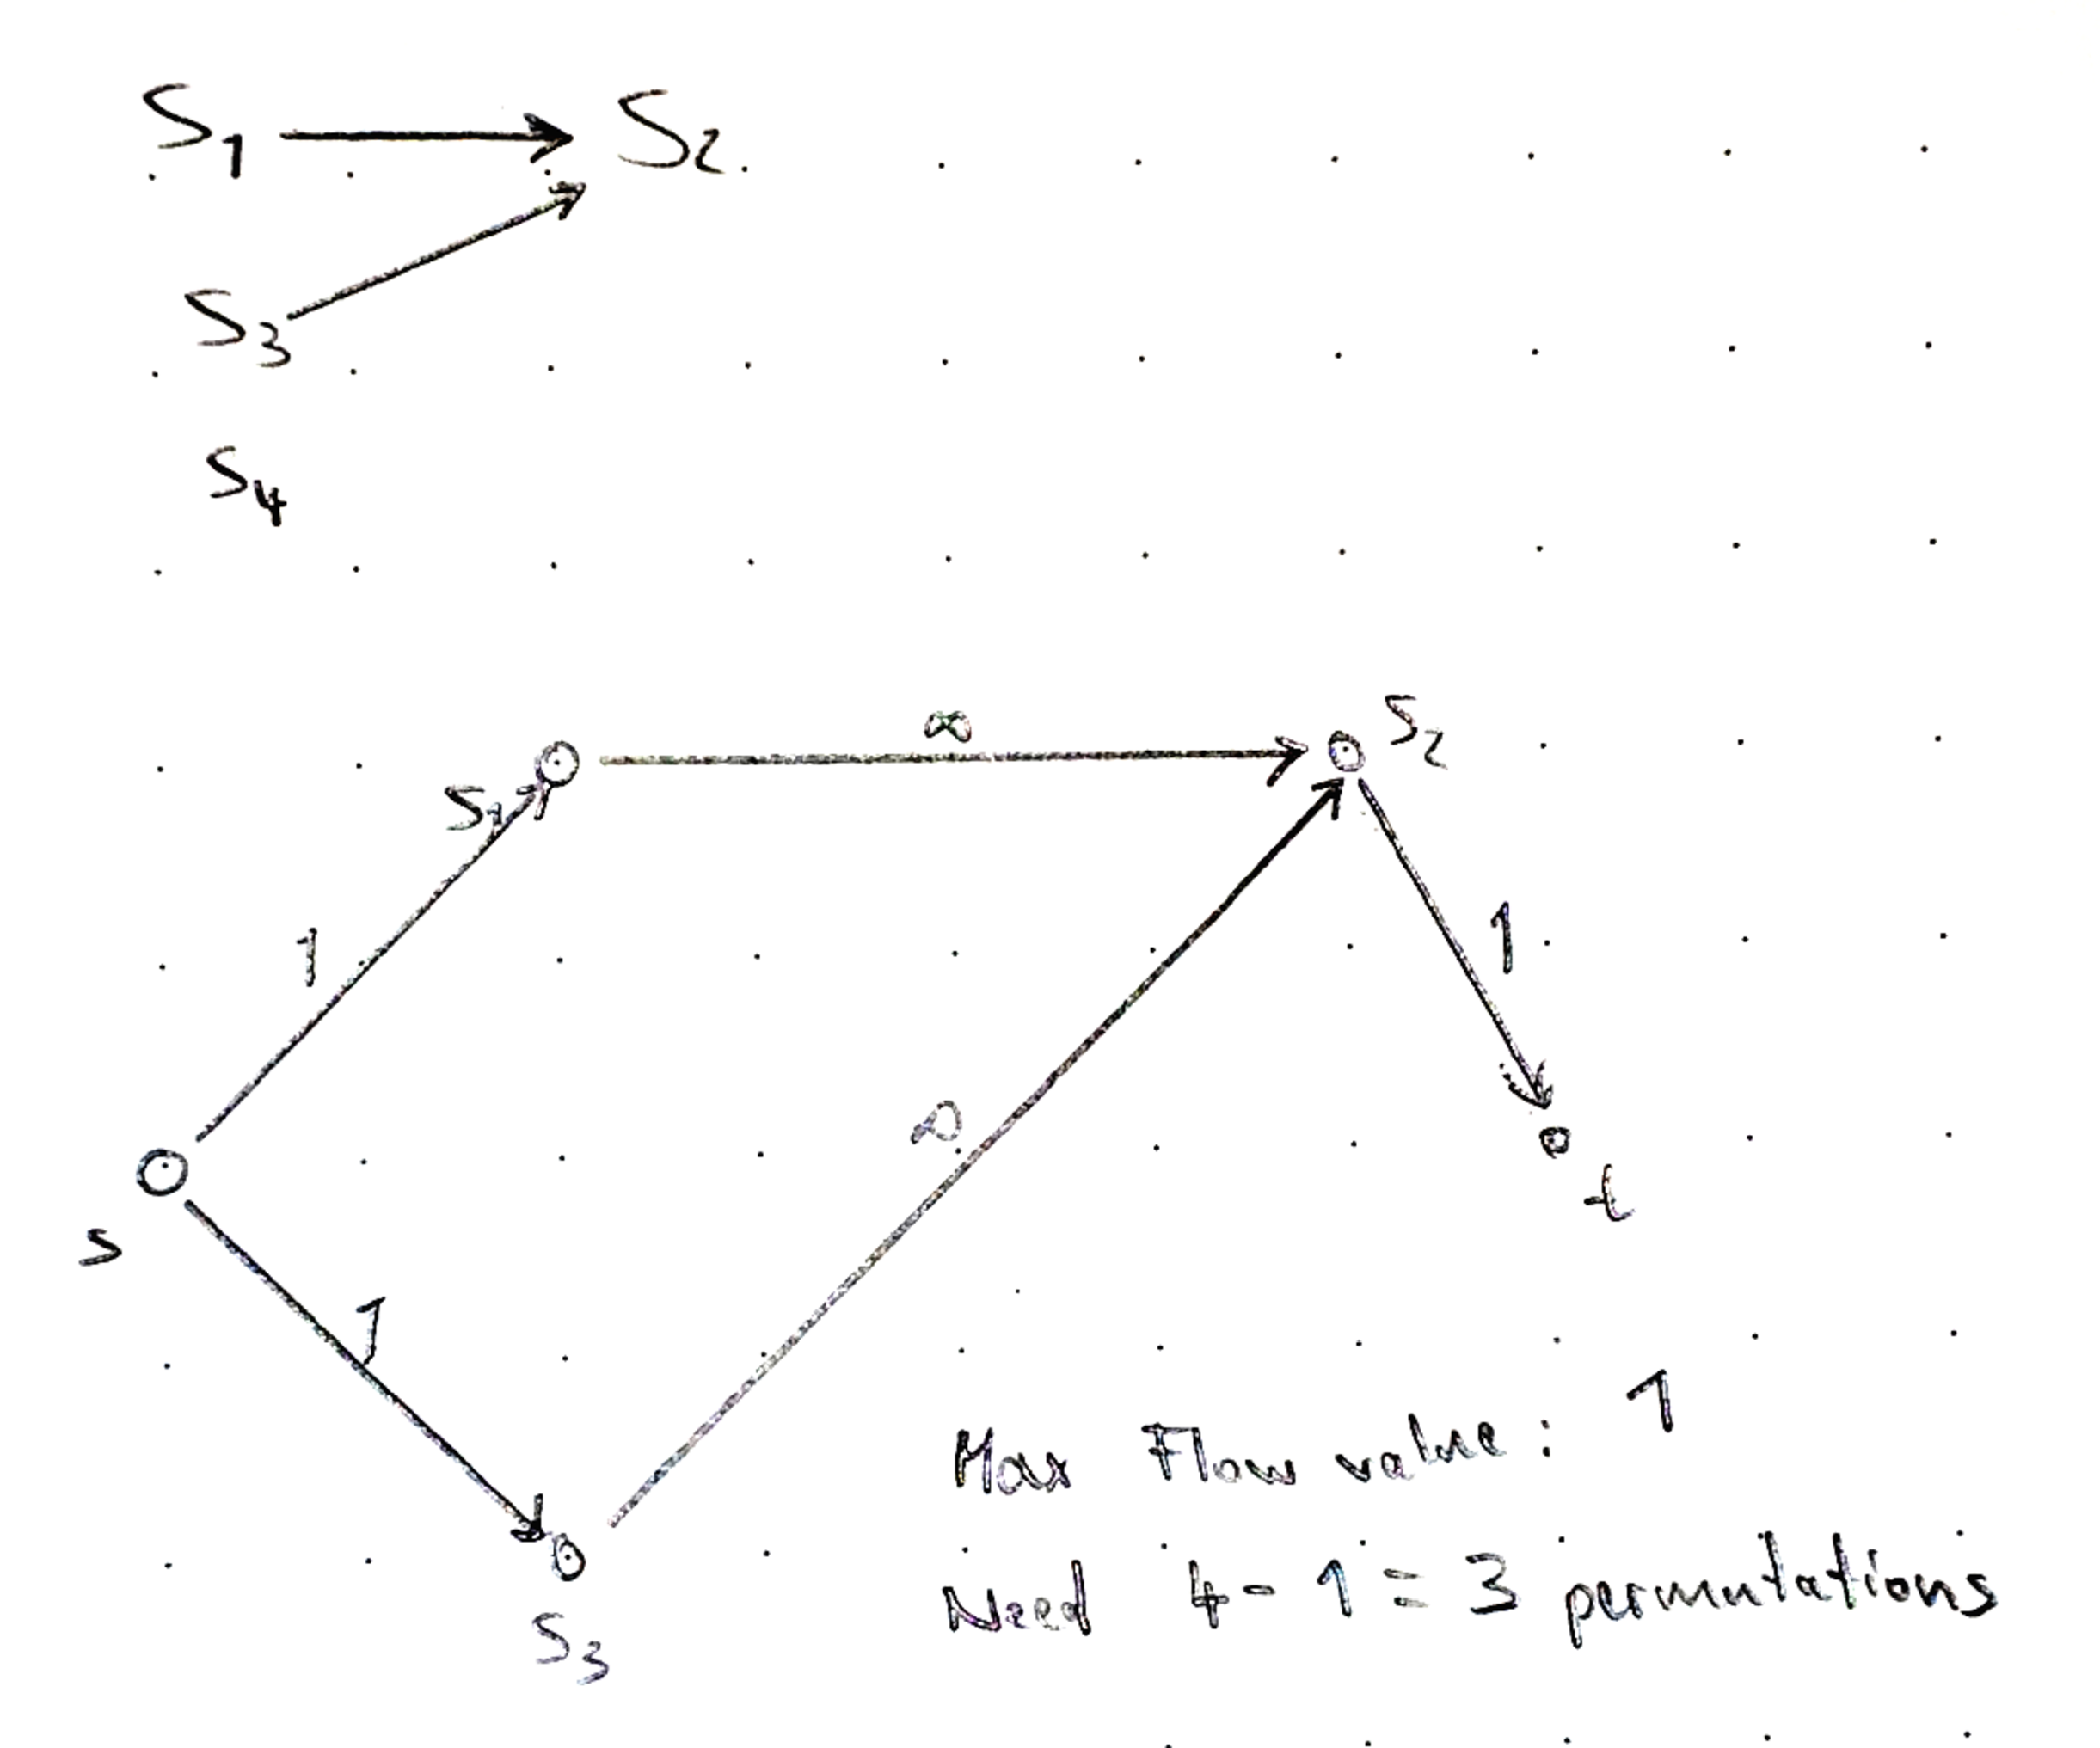
\includegraphics[width=\textwidth]{4.pdf}
\begin{itemize}
	\item We begin with a preprocessing step: for every pair of sets $S_i$ and $S_j$, we determine whether $S_i \subseteq S_j$ or $S_j \subseteq S_i$. Afterwards, we can form chains of subsets, e.g. $S_i \subseteq S_j \subseteq S_k$. In the figure above, we have the chains $(S_1, S_2)$, $(S_3, S_2)$ and $(S_4)$. We represent these chains as a graph $G=(V, E)$ as shown in the upper part of the figure. There is an edge $(S_i, S_j)$ if $S_i  \subseteq S_j$.
	\item We generate a flow network for this graph. The flow network is a bipartite graph $G' = ((V'_1 \cup V'_2), E')$ with $V'_1 = \{v \in V \left. \right| d_{\mathit{in}}(v) > 0 \}$, $V'_2 = \{v \in V \left. \right| d_\mathit{out}(v) > 0\}$, where $d_\mathit{in}(v)$ is the incoming edge degree of $v$ and $d_\mathit{out}$ is the outgoing edge degree of $v$. We connect the left part with the soruce, and the right part with the sink. There is an edge $(a,b)$ in the middle iff $a \subseteq b$.
	\item $k - \mathit{maxFlow}$ is the minimum number of permutations that we need.
	\item We can reconstruct the permutations, i.e. the subsets that correspond to one permutation by examining the flow values. Then, for every chain $(S_i, S_j, \ldots S_k)$, we can build the permutation in the following order: all columns in $S_i$, all additional columns in $S_j$, $\ldots$, all additional columns in $S_k$, all other columns in the table.
\end{itemize}

\subsection*{Flow Graph Construction}
\begin{itemize}
	\item Add a source $s$ and a sink $t$.
	\item For every $v_i \in V$, add a vertex $v_{\mathit{in},i}$ if $d_\mathit{in}(v_i) > 0$.
	\item For every $v_i \in V$, add a vertex $v_{\mathit{out},i}$ if $d_\mathit{out}(v_i) > 0$.
	\item For every $v_{\mathit{in},a} \in V'$ and $v_{\mathit{out},b} \in V'$, add an edge $(v_{\mathit{in},a}, v_{\mathit{out},b})$ with capacity $\infty$, if $a \subseteq b$.
	\item Add edges $(s, v_{\mathit{in},a})$ with capacity $1$.
	\item Add edges $(v_{\mathit{out},b},t)$ with capacity $1$.
\end{itemize}

\subsection*{Algorithm}
\begin{itemize}
	\item For every pair $S_i$, $S_j$ determine whether $S_i \subseteq S_j$ or $S_j\subseteq S_i$. This can be done by iterating over all elements in one set and checking if the element is present in the other set.
	\item Build the graph $G$: when adding the next vertex $S_i$, add an edge $(S_k, S_i)$ if $S_k \subseteq S_i$ and add an edge $(S_i, S_j)$ if $S_i \subseteq S_j$.
	\item Build the flow graph $G'$ as described in the previous subsection.
	\item If $k-\mathit{maxFlow} > l$, output \emph{no solution}.
	\item Otherwise, generate up to $l$ lists $L_i$, where $S_a$ and $S_b$ are in the same list if $f((v_{\mathit{in},a}, v_{b, \mathit{out}})) = 1$. Afterwards, every $L_i$ contains a chain, and the union of all chains is $V$i\footnote{A set $S_a$ can appear in more than just one $L_i$.}. If a set $S_c$ is not added to any list (this can happen, if there is no subset relation involving $S_c$), add it to a new list.
	\item Sort all chains by the $\subseteq$ relation, i.e. $S_a \in L_i \leq S_b \in L_i$ if $S_a \subseteq S_b$.
	\item Output a permutation for every $L_i$. The columns should be output in this sequence. Start with the first set in $L_i$ and output all its columns. For the next set in $L_i$, output all columns that were not yet output for this $L_i$ so far. Continue, until all sets are output. Output all columns of the table that were not output so far. Continue with the next $L_i$.
\end{itemize}

\subsection*{Proof}
\begin{itemize}
	\item We first show that the algorithm always generates a valid set of permutations, i.e. all permutations $T_{p_i}$ together contain all sets $S_i$ as prefixes.
	\item Every set $S_i$ is contained in some list $L_i$, because there is either a subset relation $S_j \subseteq S_i$ or a subset relation $S_j \subseteq S_i$ (then we add both to the same list), or $S_i$ is not part of a subset relation and we create a new list and $S_i$ is added to that list.
	\item After sorting the lists $L_i$, we can be sure that for $L_i = (s_1, s_2, \ldots, s_q)$ $s_{i-1} \subseteq s_i$. Therefore, if we generate the permutations in such a way that we first add the columns in $s_1$, then the columns in $s_2$, and so on, we can be sure that every $s_i$ is a prefix of the permutation. We can prove this by contradiction. Let us assume that $s_i \subseteq s_j$ and $s_j$ is a prefix of the permutation but $s_i$ is not. In that case, there must be some column out of $s_j$ in the permutation that is not in $s_i$ before finishing the enumeration of all $s_i$. But this cannot happens, because we first add all columns of $s_i$ and only then start adding additional columns from $s_j$.
	\item We can be sure that we actually generate a permutation for every $L_i$, because we add only new columns and fill up the permutation with missing columns from the table at the end.
	\item Through the minimum cut we can prove that the algorithm generates the minimum number of permutations. Therefore, we have to find the bottleneck in the network flow graph. We can be sure that, if $v_{\mathit{in}, a} \in A$, then $v_{\mathit{out},b} \in A$ if $S_a \subseteq S_b$, because these vertices are connected with an infinite edge. On the other hand, if $v_{\mathit{out}, b_1} \in A$ and $v_{\mathit{out}, b_2} \in A$, then $v_{\mathit{in}, a} \in A$ if $S_a \subseteq S_{b_1}$ and $S_a \subseteq S_{b_2}$ because, otherwise, we could reduce the max flow by $1$ by adding $v_{\mathit{in},a}$ to $A$. We can show that the min cut value is the number of sets, for which we can reuse or extend an existing chain. Therefore, $k-\mathit{maxFlow}$ is the number of times we have to use a new chain. This obviously has to be true for at least one set, because we need at least one permutation.
\end{itemize}

\subsection*{Runtime}
\begin{itemize}
	\item Determining subset relation for every pair of sets: we have to check if each element is present in the other set. This can be done in $\mathcal{O}(n \cdot k^2)$.
	\item Building the graph $G$: we add $k$ vertices and up to $k^2$ edges, therefore the runtime is $\mathcal{O}(k^2)$.
	\item Building the flow network $G'$: we add $2k$ vertices and up to $(2k)^2$ edges, therefore the runtime is $\mathcal{O}(k^2)$.
	\item The max flow can be determined with the Edmonds-Karp algorithm in $\mathcal{O}(|V| |E|^2) = \mathcal{O}(k^5)$.
	\item Creating the lists $L_i$: we add up to $\mathcal{O}(2 k^2)$ vertices to the lists $L_i$.
	\item Sorting all $L_i$: there are no more than $l$ lists, so the runtime is $\mathcal{O}(l \cdot (k^2 \log k^2)) = \mathcal{O}(k \cdot (k^2 \log k^2))$ because $l < k$.
	\item Output all permutations: there are $\mathcal{O}(k^2)$ sets in total in all $L_i$, and every set can contain up to $n$ elements. Therefore, the runtime is $\mathcal{O}(n k^2)$. To check whether we already output a column, we can use a hash set with constant insertion/accessing runtime (for $n$ elements: no more than $\mathcal{O}(n)$).
	\item The overall runtime of the algorithm is $\mathcal{O}(\max \{n \cdot k^2, k^5 \})$.
\end{itemize}
\end{document}

